%%%%%%%%%%%%%%%%%%%%%%%%%%%%%%%%%%%%%%%%
% datoteka diploma-vzorec.tex
%
% vzorčna datoteka za pisanje diplomskega dela v formatu LaTeX
% na UL Fakulteti za računalništvo in informatiko
%
% vkup spravil Gašper Fijavž, december 2010
% 
%
%
% verzija 12. februar 2014 (besedilo teme, seznam kratic, popravki Gašper Fijavž)
% verzija 10. marec 2014 (redakcijski popravki Zoran Bosnić)
% verzija 11. marec 2014 (redakcijski popravki Gašper Fijavž)
% verzija 15. april 2014 (pdf/a 1b compliance, not really - just claiming, Damjan Cvetan, Gašper Fijavž)
% verzija 23. april 2014 (privzeto cc licenca)
% verzija 16. september 2014 (odmiki strain od roba)
% verzija 28. oktober 2014 (odstranil vpisno številko)
% verija 5. februar 2015 (Literatura v kazalu, online literatura)
% verzija 25. september 2015 (angl. naslov v izjavi o avtorstvu)
% verzija 26. februar 2016 (UL izjava o avtorstvu)
% verzija 16. april 2016 (odstranjena izjava o avtorstvu)
% verzija 5. junij 2016 (Franc Solina dodal vrstice, ki jih je označil s svojim imenom)

% \UseRawInputEncoding
\documentclass[a4paper, 12pt]{book}
%\documentclass[a4paper, 12pt, draft]{book}  Nalogo preverite tudi z opcijo draft, ki vam bo pokazala, katere vrstice so predolge!


\usepackage[utf8]{inputenc}   % omogoča uporabo slovenskih črk kodiranih v formatu UTF-8
\usepackage[slovene,english]{babel}    % naloži, med drugim, slovenske delilne vzorce

\usepackage[
backend=biber,
maxbibnames=9,
]{biblatex}

% If you want to break on URL numbers
\setcounter{biburlnumpenalty}{9000}
% If you want to break on URL lower case letters
\setcounter{biburllcpenalty}{9000}
% If you want to break on URL UPPER CASE letters
\setcounter{biburlucpenalty}{9000}

\addbibresource{literatura.bib}

\usepackage[pdftex]{graphicx}  % omogoča vlaganje slik različnih formatov
\graphicspath{ {./images/} }

\usepackage{float}          % poskrbi, na primer, za glave strani
\usepackage{csquotes}
\DeclareQuoteAlias{german}{english}
\usepackage{fancyhdr}          % poskrbi, na primer, za glave strani
\usepackage{fancyvrb}          % poskrbi za underlined verbatim
\usepackage{amssymb}           % dodatni simboli
\usepackage{amsmath}           % eqref, npr.
\usepackage{hyperxmp}
%\usepackage[hyphens]{url}  % dodal Solina
%\usepackage{comment}       % dodal Solina
\usepackage[pdftex, colorlinks=true,
  						citecolor=black, filecolor=black, 
  						linkcolor=black, urlcolor=black,
  						pagebackref=false, 
  						pdfproducer={LaTeX}, pdfcreator={LaTeX}, hidelinks]{hyperref}
 
%\usepackage[separate-uncertainty=true,multi-part-units=repeat]{siunitx}

\usepackage{color}       % dodal Solina
\usepackage{soul}       % dodal Solina

%%%%%%%%%%%%%%%%%%%%%%%%%%%%%%%%%%%%%%%%
%	DIPLOMA INFO
%%%%%%%%%%%%%%%%%%%%%%%%%%%%%%%%%%%%%%%%
\newcommand{\ttitle}{Avtomatizacija delavniškega dnevnika}
\newcommand{\ttitleEn}{Workshop report automatization}
\newcommand{\tsubject}{\ttitle}
\newcommand{\tsubjectEn}{\ttitleEn}
\newcommand{\tauthor}{Anej Lekše}
\newcommand{\tkeywords}{mobilni razvoj, glasovni pomočniki, razpoznava glasu, informacijski sistemi}
\newcommand{\tkeywordsEn}{mobile development, voice assistants, voice recognition, information systems}


%%%%%%%%%%%%%%%%%%%%%%%%%%%%%%%%%%%%%%%%
%	HYPERREF SETUP
%%%%%%%%%%%%%%%%%%%%%%%%%%%%%%%%%%%%%%%%
\hypersetup{pdftitle={\ttitle}}
\hypersetup{pdfsubject=\ttitleEn}
\hypersetup{pdfauthor={\tauthor, al1617@student.uni-lj.si}}
\hypersetup{pdfkeywords=\tkeywordsEn}


 


%%%%%%%%%%%%%%%%%%%%%%%%%%%%%%%%%%%%%%%%
% postavitev strani
%%%%%%%%%%%%%%%%%%%%%%%%%%%%%%%%%%%%%%%%  

\addtolength{\marginparwidth}{-20pt} % robovi za tisk
\addtolength{\oddsidemargin}{40pt}
\addtolength{\evensidemargin}{-40pt}

\renewcommand{\baselinestretch}{1.3} % ustrezen razmik med vrsticami
\setlength{\headheight}{15pt}        % potreben prostor na vrhu
\renewcommand{\chaptermark}[1]%
{\markboth{\MakeUppercase{\thechapter.\ #1}}{}} \renewcommand{\sectionmark}[1]%
{\markright{\MakeUppercase{\thesection.\ #1}}} \renewcommand{\headrulewidth}{0.5pt} \renewcommand{\footrulewidth}{0pt}
\fancyhf{}
\fancyhead[LE,RO]{\sl \thepage} 
%\fancyhead[LO]{\sl \rightmark} \fancyhead[RE]{\sl \leftmark}
\fancyhead[RE]{\sc \tauthor}              % dodal Solina
\fancyhead[LO]{\sc Diplomska naloga}     % dodal Solina


\newcommand{\BibTeX}{{\sc Bib}\TeX}

%%%%%%%%%%%%%%%%%%%%%%%%%%%%%%%%%%%%%%%%
% naslovi
%%%%%%%%%%%%%%%%%%%%%%%%%%%%%%%%%%%%%%%%  


\newcommand{\autfont}{\Large}
\newcommand{\titfont}{\LARGE\bf}
\newcommand{\clearemptydoublepage}{\newpage{\pagestyle{empty}\cleardoublepage}}
\setcounter{tocdepth}{1}	      % globina kazala

%%%%%%%%%%%%%%%%%%%%%%%%%%%%%%%%%%%%%%%%
% konstrukti
%%%%%%%%%%%%%%%%%%%%%%%%%%%%%%%%%%%%%%%%  
\newtheorem{izrek}{Izrek}[chapter]
\newtheorem{trditev}{Trditev}[izrek]
\newenvironment{dokaz}{\emph{Dokaz.}\ }{\hspace{\fill}{$\Box$}}

%%%%%%%%%%%%%%%%%%%%%%%%%%%%%%%%%%%%%%%%%%%%%%%%%%%%%%%%%%%%%%%%%%%%%%%%%%%%%%%
%% PDF-A
%%%%%%%%%%%%%%%%%%%%%%%%%%%%%%%%%%%%%%%%%%%%%%%%%%%%%%%%%%%%%%%%%%%%%%%%%%%%%%%


%%%%%%%%%%%%%%%%%%%%%%%%%%%%%%%%%%%%%%%% 
% define medatata
%%%%%%%%%%%%%%%%%%%%%%%%%%%%%%%%%%%%%%%% 
\def\Title{\ttitle}
\def\Author{\tauthor, al1617@student.uni-lj.si}
\def\Subject{\ttitleEn}
\def\Keywords{\tkeywordsEn}

%%%%%%%%%%%%%%%%%%%%%%%%%%%%%%%%%%%%%%%% 
% \convertDate converts D:20080419103507+02'00' to 2008-04-19T10:35:07+02:00
%%%%%%%%%%%%%%%%%%%%%%%%%%%%%%%%%%%%%%%% 
\def\convertDate{%
    \getYear
}

{\catcode`\D=12
 \gdef\getYear D:#1#2#3#4{\edef\xYear{#1#2#3#4}\getMonth}
}
\def\getMonth#1#2{\edef\xMonth{#1#2}\getDay}
\def\getDay#1#2{\edef\xDay{#1#2}\getHour}
\def\getHour#1#2{\edef\xHour{#1#2}\getMin}
\def\getMin#1#2{\edef\xMin{#1#2}\getSec}
\def\getSec#1#2{\edef\xSec{#1#2}\getTZh}
\def\getTZh +#1#2{\edef\xTZh{#1#2}\getTZm}
\def\getTZm '#1#2'{%
    \edef\xTZm{#1#2}%
    \edef\convDate{\xYear-\xMonth-\xDay T\xHour:\xMin:\xSec+\xTZh:\xTZm}%
}

\expandafter\convertDate\pdfcreationdate 

%%%%%%%%%%%%%%%%%%%%%%%%%%%%%%%%%%%%%%%%
% get pdftex version string
%%%%%%%%%%%%%%%%%%%%%%%%%%%%%%%%%%%%%%%% 
\newcount\countA
\countA=\pdftexversion
\advance \countA by -100
\def\pdftexVersionStr{pdfTeX-1.\the\countA.\pdftexrevision}


%%%%%%%%%%%%%%%%%%%%%%%%%%%%%%%%%%%%%%%%
% XMP data
%%%%%%%%%%%%%%%%%%%%%%%%%%%%%%%%%%%%%%%%  
\usepackage{xmpincl}
\includexmp{pdfa-1b}

%%%%%%%%%%%%%%%%%%%%%%%%%%%%%%%%%%%%%%%%
% pdfInfo
%%%%%%%%%%%%%%%%%%%%%%%%%%%%%%%%%%%%%%%%  
\pdfinfo{%
    /Title    (\ttitle)
    /Author   (\tauthor, damjan@cvetan.si)
    /Subject  (\ttitleEn)
    /Keywords (\tkeywordsEn)
    /ModDate  (\pdfcreationdate)
    /Trapped  /False
}


%%%%%%%%%%%%%%%%%%%%%%%%%%%%%%%%%%%%%%%%%%%%%%%%%%%%%%%%%%%%%%%%%%%%%%%%%%%%%%%
%%%%%%%%%%%%%%%%%%%%%%%%%%%%%%%%%%%%%%%%%%%%%%%%%%%%%%%%%%%%%%%%%%%%%%%%%%%%%%%

\begin{document}
\selectlanguage{slovene}
\frontmatter
\setcounter{page}{1} %
\renewcommand{\thepage}{}       % preprecimo težave s številkami strani v kazalu
\newcommand{\sn}[1]{"`#1"'}                    % dodal Solina (slovenski narekovaji)

%%%%%%%%%%%%%%%%%%%%%%%%%%%%%%%%%%%%%%%%
%naslovnica
 \thispagestyle{empty}%
   \begin{center}
    {\large\sc Univerza v Ljubljani\\%
      Fakulteta za računalništvo in informatiko}%
    \vskip 10em%
    {\autfont \tauthor\par}%
    {\titfont \ttitle \par}%
    {\vskip 3em \textsc{DIPLOMSKO DELO\\[5mm]         % dodal Solina za ostale študijske programe
    VISOKOŠOLSKI STROKOVNI ŠTUDIJSKI PROGRAM\\ PRVE STOPNJE\\ RAČUNALNIŠTVO IN INFORMATIKA}\par}%
%    UNIVERZITETNI  ŠTUDIJSKI PROGRAM\\ PRVE STOPNJE\\ RAČUNALNIŠTVO IN INFORMATIKA}\par}%
%    INTERDISCIPLINARNI UNIVERZITETNI\\ ŠTUDIJSKI PROGRAM PRVE STOPNJE\\ RAČUNALNIŠTVO IN MATEMATIKA}\par}%
%    INTERDISCIPLINARNI UNIVERZITETNI\\ ŠTUDIJSKI PROGRAM PRVE STOPNJE\\ UPRAVNA INFORMATIKA}\par}%
%    INTERDISCIPLINARNI UNIVERZITETNI\\ ŠTUDIJSKI PROGRAM PRVE STOPNJE\\ MULTIMEDIJA}\par}%
    \vfill\null%
    {\large \textsc{Mentor}: dr.  Andrej Brodnik\par}%
   %{\large \textsc{Somentor}:  izr.\ prof.\ dr. Martin Krpan \par}%
    {\vskip 2em \large Ljubljana, 2020 \par}%
\end{center}
% prazna stran
%\clearemptydoublepage      % dodal Solina (izjava o licencah itd. se izpiše na hrbtni strani naslovnice)

%%%%%%%%%%%%%%%%%%%%%%%%%%%%%%%%%%%%%%%%
%copyright stran
\thispagestyle{empty}
\vspace*{8cm}

\noindent
{\sc Copyright}. 
Rezultati diplomske naloge so intelektualna lastnina avtorja in Fakultete za računalništvo in informatiko Univerze v Ljubljani.
Za objavo in koriščenje rezultatov diplomske naloge je potrebno pisno privoljenje avtorja, Fakultete za računalništvo in informatiko ter mentorja.

\begin{center}
\mbox{}\vfill
\emph{Besedilo je oblikovano z urejevalnikom besedil \LaTeX.}
\end{center}
% prazna stran
\clearemptydoublepage

%%%%%%%%%%%%%%%%%%%%%%%%%%%%%%%%%%%%%%%%
% stran 3 med uvodnimi listi
\thispagestyle{empty}
\vspace*{4cm}

\noindent
Fakulteta za računalništvo in informatiko izdaja naslednjo nalogo:
\medskip
\begin{tabbing}
\hspace{32mm}\= \hspace{6cm} \= \kill




Tematika naloge:
\end{tabbing}
%Besedilo teme diplomskega dela študent prepiše iz študijskega informacijskega sistema, kamor ga je vnesel mentor. V nekaj stavkih bo opisal, kaj pričakuje od kandidatovega diplomskega dela. Kaj so cilji, kakšne metode uporabiti, morda bo zapisal tudi ključno literaturo.
Preveri, ali so glasovni pomočniki v trenutnem stanju primerni za pomoč pri pisanju delavniških dnevnikov.
Seznani se z obstoječimi rešitvami za sestavljanje delavniških dnevnikov in jih analiziraj.
Po analizi področja se loti izdelave svojega sistema za sestavljanje delavniških dnevnikov, ki vključuje glasovnega pomočnika.
\vspace{15mm}



\vspace{2cm}

% prazna stran
\clearemptydoublepage

% zahvala
\thispagestyle{empty}\mbox{}\vfill\null\it%
\noindent
Zahvaljujem se očetu in mami za neizmerno podporo, podjetju Hisense Gorenje Europe za slikovno gradivo in pomoč.
Roku Bermežu.

Hvala vsem.
\rm\normalfont

% prazna stran
\clearemptydoublepage

%%%%%%%%%%%%%%%%%%%%%%%%%%%%%%%%%%%%%%%%
% posvetilo, če sama zahvala ne zadošča :-)
\thispagestyle{empty}\mbox{}{\vskip0.20\textheight}\mbox{}\hfill\begin{minipage}{0.55\textwidth}%
% Svoji dragi Alenčici.
	Kavi. Tii. Hvala.
\normalfont\end{minipage}

% prazna stran
\clearemptydoublepage


%%%%%%%%%%%%%%%%%%%%%%%%%%%%%%%%%%%%%%%%
% kazalo
\pagestyle{empty}
\def\thepage{}% preprecimo tezave s stevilkami strani v kazalu
\tableofcontents{}


% prazna stran
\clearemptydoublepage

%%%%%%%%%%%%%%%%%%%%%%%%%%%%%%%%%%%%%%%%
% seznam kratic

\chapter*{Seznam uporabljenih kratic}  % spremenil Solina, da predolge vrstice ne gredo preko desnega roba

% \begin{comment}
% \begin{tabular}{l|l|l}
%   {\bf kratica} & {\bf angleško} & {\bf slovensko} \\ \hline
%   % after \\: \hline or \cline{col1-col2} \cline{col3-col4} ...
%   {\bf CA} & classification accuracy & klasifikacijska točnost \\
%   {\bf DBMS} & database management system & sistem za upravljanje podatkovnih baz \\
%   {\bf SVM} & support vector machine & metoda podpornih vektorjev \\
%   \dots & \dots & \dots \\
% \end{tabular}
% \end{comment}

\noindent\begin{tabular}{p{0.1\textwidth}|p{.4\textwidth}|p{.4\textwidth}}    % po potrebi razširi prvo kolono tabele na račun drugih dveh!
  {\bf kratica} & {\bf angleško}                             & {\bf slovensko} \\ \hline
  {\bf API} & Application Programming Interface & Vmesnik za programiranje aplikacije \\
  {\bf AWS} & Amazon Web Services & Amazonove spletne storitve \\
  {\bf FIFO} & First In First Out & Prvi not, prvi ven \\
  {\bf HTML} & HyperText Markup Language & Označitveni jezik za hipertekst \\
  {\bf HTTP} & HyperText Transfer Protocol & Protokol za prenos hiperteksta \\
  % {\bf HTTPS} & HyperText Transfer Protocol Secure & Protokol za prenos hiperteksta, varna različica? \\
  {\bf IP} & Internet Protocol & Internetni protokol \\
  {\bf JSON} & JavaScript Object Notation & JavaScript zapis objektov\\
  {\bf JWT} & JSON Web Token & JSON spletni žeton \\
  % {\bf LIMS} & Laboratory Information Management System & laboratorijski sistem za uporavljanje informacij \\
  {\bf MIT} & Massachusetts Institute of Technology & Tehnološki inštitut Massachusettsa \\
  {\bf MVVM} & Model View View-Model & Model Pogled Pogled-Model \\
  {\bf NLU} & Natural Langugage Understanding & Razumevanje naravnega govora \\
  {\bf SQS} & Simple Queue Service & Preprosta vrstna storitev \\
  {\bf UI} & User Interface & Uporabniški vmesnik \\
  {\bf URL} & Universal Resource Locator & Univerzalni lokator virov \\
  %  {\bf VUI} & Voice User Interface & glasovni uporabniški vmesnik \\
  {\bf XAML} & Extensible Application Markup Langugage & Razširljiv aplikacijski označitveni jezik \\
%  \dots & \dots & \dots \\
\end{tabular}


% prazna stran
\clearemptydoublepage

%%%%%%%%%%%%%%%%%%%%%%%%%%%%%%%%%%%%%%%%
% povzetek
\addcontentsline{toc}{chapter}{Povzetek}
\chapter*{Povzetek}

\noindent\textbf{Naslov:} \ttitle
\bigskip

\noindent\textbf{Avtor:} \tauthor
\bigskip

%Dober povzetek vključuje: (1) kratek opis obravnavanega problema, (2) kratek opis vašega pristopa za reševanje tega problema in (3) (najbolj uspešen) rezultat ali prispevek magistrske naloge.

\noindent Diplomsko delo obravnava področje vpeljave komercialno dostopnih glasovnih pomočnikov v programske rešitve kot dodatni uporabniški vmesnik.
V nalogi raziščemo, kako v računalniški sistem vpeljemo glasovnega pomočnika in vpliv glasovnega pomočnika na uporabo sistema.
% V nalogi raziščemo, kako vpeljava glasovnega pomočnika v računalniški sistem pospeši delo s tem sistemom. 
Cilj je implementirati in preizkusiti računalniški sistem z glasovnim pomočnikom, s pomočjo katerega lahko narekujemo zapiske med delom. 
Te zapiske pa lahko naknandno urejamo s pomočjo mobilne aplikacije.
Uporabili smo Amazon Alexo zaradi enostavne izdelave lastnih programov z Alexa Skills Kit ogrodjem.
% Ugotovili smo, da je specializiran sistem za pisanje opisov tehnološkega postopka lahko dobra alternativa pisanju teh dokumentov s pisarniškimi programi ali na list papirja.
Ugotovili smo, da Amazon Alexa ni bila zmožna razpoznati izgovorjenih stavkov z veliko variirajočimi besedami.
Uspešna je bila pri razpoznavanju stavkov, ki so se v celoti ujemali z naučenim razpoznavnim modelom.
Kljub temu je čas, ki je potreben, da Alexa razpozna prejet glasovni ukaz prepočasen, da bi bil sistem, v času raziskave, učinkovit.
\bigskip

\noindent\textbf{Ključne besede:} \tkeywords.
% prazna stran
\clearemptydoublepage

%%%%%%%%%%%%%%%%%%%%%%%%%%%%%%%%%%%%%%%%
% abstract
\selectlanguage{english}
\addcontentsline{toc}{chapter}{Abstract}
\chapter*{Abstract}

\noindent\textbf{Title:} \ttitleEn
\bigskip

\noindent\textbf{Author:} \tauthor
\bigskip

\noindent This thesis deals with the process of incorporating a commercially available voice assistant into a software solution as an additional user interface.
We research how to implement a voice assistant in a software solution and how it effects its workflow.
The goal of this thesis is implementing and testing a system with a voice assistant that could be used to write workshop report steps during work.
These steps can later be edited with a mobile application.
We have used Amazon Alexa, as it offers simple programming with Alexa Skills Kit.
% We discovered that a specialised system for writing workshop reports can be an improvement over writing them with office suites or using pen and paper.
We found that Amazon Alexa was unsuitable for literal dictation of longer, varying text.
It was successful at recognising phrases that fully or mostly matched its learned model.
Regardless, Alexa's ability to process third party voice commands, at the time of this research, was too slow to be deemed efficient.

\bigskip

\noindent\textbf{Keywords:} \tkeywordsEn.
\selectlanguage{slovene}
% prazna stran
\clearemptydoublepage

%%%%%%%%%%%%%%%%%%%%%%%%%%%%%%%%%%%%%%%%
\mainmatter
\setcounter{page}{1}
\pagestyle{fancy}

\chapter{Uvod}
\section{Opis domene raziskave}

Diplomsko delo obravnava področje vpeljave glasovnih pomočnikov v programske rešitve kot dodatni uporabniški vmesnik.

Za področje, ki ga želimo z našo rešitvijo  izboljšati, smo si izbrali sestavljanje delavniškega dnevnika (v nadaljevanju imenovanega tudi opisa tehnološkega postopka).
Kljub temu se bo naš sistem, lahko uporabil tudi za sestavljanje drugačnih vrst poročil in navodil.
Med te spadajo na primer kuharski recepti, laboratorijski dnevniki, itd.

Opis tehnološkega postopka ali delavniški dnevnik je dokument, ki po korakih predstavi postopek izdelave izdelka.
Delavniški dnevniki imajo lahko definirane tudi kontrolne postopke za izdelek, orodje, ki ga rabimo za izdelavo, in seznam možnih nevarnosti pri delu.

Delavniški dnevnik je sestavljen iz zaporedja korakov, ki si sledijo v časovnem zaporedju.
Vsak korak sestavljata opis postopka in predvideno trajanje.
Koraki lahko vsebujejo tudi slikovne razlage.

Opisi tehnološkega postopka se najpogosteje uporabljajo v proizvodnih obratih tovarn kot navodila in oporne točke za sestavljalce.

V sklopu diplomske naloge smo želeli izdelati specializiran sistem za sestavljanje delavniških dnevnikov, nato pa preveriti, ali lahko z vpeljavo glasovnega pomočnika delo s tem sistemom izboljšamo.
Ta sistem bi sestavljali glasovni pomočnik, ki bi služil za narekovanje opomb, mobilna aplikacija, preko katere bi lahko urejali zapiske in strežnik, ki bi hranil podatke.
% Ta sistem bi sestavljali strežnik, ki bi hranil podatke o delavniških dnevnikih, mobilna aplikacija, preko katere bi uporabnik do teh podatkov dostopal in glasovni pomočnik, s katerim bi lahko dobesedno narekovali korake in nadzirali mobilno aplikacijo.

Raziskati želimo, kako vpeljati glasovnega asistenta Amazon Alexo v programsko rešitev in kako vpeljava Alexe vpliva na interakcijo uporabnika s sistemom.


\section{Struktura diplomske naloge}

Diplomsko delo pričenjamo s predstavitvijo področja raziskave in kratko opišemo problem in možno rešitev. 
Opredelimo problematiko naše raziskave.

Začnemo z raziskavo obstoječih rešitev za sestavljanje opisa tehnološkega postopka.
Nato opišemo, kaj trenutne rešitve te problematike ponujajo in poskusimo opredeliti njihove prednosti ter slabosti.

V naslednjem poglavju se lotimo načrtovanja specializiranega sistema z glasovnim pomočnikom za pomoč pri pisanju delavniških dnevnikov.
Nato se lotimo opisa tehnologij, ki smo jih pri pisanju diplome uporabili.
Natančno definiramo funkcionalnosti sistema, utemeljimo odločitev za izbiro Amazon Alexe, AWS Simple Queue Service, AWS Lambda in ogrodja Xamarin.

Nato predstavimo Alexa \enquote{Skill}, strežniški program in mobilno aplikacijo.
Funkcionalnosti sistema testiramo.

V zadnjem poglavju opišemo možnosti nadaljnjega razvoja projekta.

\chapter{Pregled problema in rešitve}

\section{Problem}

\subsection {Kaj vsebuje delavniški dnevnik?}

Delavniški dnevnik je splošen izraz za tehniški dokument, ki po korakih predstavi potek tehnološkega postopka \cite{delavniskidnevnikptuj}.
V podjetju Hisense Gorenje Europe takšne dokumente imenujejo opis tehnološkega postopka (slika \ref{sap_2}).

Delavniški dnevnik sestavlja zaporedje korakov, ki si sledijo v časovnem vrstnem redu.
Vsak korak delavniškega dnevnika sestavljata opis postopka posamezne naloge v procesu in njeno predvideno trajanje.
Delavniški dnevniki lahko vsebujejo tudi slikovne razlage.

Delavniški dnevniki imajo lahko definirane tudi kontrolne postopke za izdelek, orodje, ki ga potrebujemo za izdelavo in seznam možnih nevarnosti pri delu.

Delavniški dnevniki se uporabljajo v proizvodnih obratih tovarn kot navodila in oporne točke za sestavljalce.
Pogosto se uporabljajo tudi kot učni pripomoček za spremljanje napredka npr. dijakov vajencev na praksi \cite{delavniskidnevnikptuj, ddsclj}.

\begin{figure}[H]
\begin{center}
\includegraphics[width=13.5cm]{sap_2}
\end{center}
\caption{V tabelo izvožen opis tehnološkega postopka za izdelavo hladilnika v podjetju Hisense Gorenje Europe}
\label{sap_2}
\end{figure}

% Ta opis tehnološkega postopka je strukturiran tako, da se vsi koraki sklicujejo na eno samo tehnično sliko.

% // kako podrobno se opisuje korake?

Delavniški dnevnik se lahko sestavlja med delom ali po opravljenem delu.

\subsection{Definicija problematike}

V tej diplomski nalogi raziščemo možne metode izdelave delavniškega dnevnika oz. opisa tehnološkega postopka.
Raziskati želimo prednosti in slabosti trenutnih metod sestavljanja teh dokumentov.
V naslednji fazi raziskave želimo izdelati specializiran sistem za sestavljanje opisov tehnoloških postopkov.
Raziskati želimo vpeljavo glasovnega pomočnika v sistem za sestavljanje delavniških dnevnikov in kako uporaba glasovnega pomočnika vpliva na uporabo takega sistema.


Izhajajoč iz navedenega opredeljujemo problematiko diplomskega dela: zasnuj in implementiraj sistem za sestavljanje delavniških dnevnikov, vanj vpelji glasovnega pomočnika in sistem preizkusi.

\section{Obstoječe rešitve}

\subsection{Papir in pisalo}

Najstarejša metoda za izdelavo takšnega dokumenta je zapis na list papirja (slika \ref{paper}).

\begin{figure}[H]
\begin{center}
\includegraphics[width=13.5cm]{report_paper_small}
\end{center}
\caption{Opis tehnološkega postopka za čiščenje tipkovnice na papirju.}
\label{paper}
\end{figure}


Prednosti uporabe papirja in pisala so, da pri delu izdelovalec ne potrebuje računalnika in cenovna ugodnost.
Slabosti takšnega postopka so:
\begin{itemize}
	\item omejitve glede velikosti prostora, namenjenega vsakemu koraku,
	\item problematično dopisovanje in urejanje obstoječih korakov,
	\item zahtevnejše arhiviranje od računalniških datotek,
	\item občutljivost papirja na fizične poškodbe (trganje, mečkanje, vnetljivost,...).
\end{itemize}

% V sklopu diplomske naloge smo na papir napisali preprost opis tehnološkega postopka (slika \ref{paper}).
% Priprava formularja je trajala 10 minut.
% Pisanje dokumenta je trajalo 7 minut.

\subsection{Pisarniški programi}

Opis tehnološkega postopka lahko izdelamo v pisarniških programih, na primer Microsoft Word ali LibreOffice Writer.

Ta pristop reši nekatere slabosti uporabe papirja in pisala za sestavljanje opisa tehnološkega postopka.
Korake lahko enostavno dodajamo in urejamo.
Prav tako je možno dodajati slikovno gradivo.
Pisarniški programi omogočajo izpis dokumenta na tiskalnik, če želimo imeti dokument natisnjen na papirju.

Kljub temu uporaba te metode prinese nove slabosti:
\begin{itemize}
	\item če imamo dokument shranjen na več mestih, moramo ob spremembah zagotoviti, da se spremenijo vse shranjene različice. 
	\item Slikovno gradivo je vezano na dokument. Ob spremembah moramo spremeniti celoten dokument, ne le slike.
	\item Možnost izgube ali izbrisa podatkov.
\end{itemize}

V sklopu diplomske naloge smo napisali preprost opis tehnološkega postopka (slika \ref{report_writer}) s programom LibreOffice Writer \cite{writer}.
% Priprava formularja je trajala 10 minut.
% Pisanje in urejanje dokumenta je trajalo 4 minute.
% Enostavno ga je bilo izvoziti v format PDF.
Dokument brez vsebine se lahko pri naslednjem opisu uporabi kot obrazec.

\begin{figure}[H]
\begin{center}
\includegraphics[width=13cm]{report_writer}
\end{center}
\caption{Preprost opis tehnološkega postopka za čiščenje tipkovnice, napisan v pisarniškem programu.}
\label{report_writer}
\end{figure}

\subsection{Specializirani moduli za poslovne informacijske sisteme}

Podjetja kot so npr. Hisense Gorenje Europe, za sestavljanje delavniških dnevnikov uporabljajo specializirane module za lastne informacijske sisteme.
Primer je prikazan modul za informacijski sistem SAP (na sliki \ref{sap_1}).

\begin{figure}[H]
\begin{center}
\includegraphics[width=13cm]{sap_1}
\end{center}
\caption{Prikazan korak opisa tehnološkega postopka s programom SAP.}
\label{sap_1}
\end{figure}

Do tega opisa tehnološkega postopka se lahko dostopa iz računalnikov na delovnih mestih, kjer se izvajajo koraki, opisani v dokumentu.
Opis tehnološkega postopka v sistemu SAP sestavljajo:
\begin{itemize}
	\item podatki o izdelku,
	\item dodatne opombe,
	\item opisi korakov,
	\item definicija kontrolnih postopkov in pregleda, 
	\item CAD izris izdelka.
\end{itemize}

Specializiran informacijski sistem, kot je SAP, je tesno povezan s proizvodno linijo in prilagodljiv za potrebe proizvodnega obrata, ki ga uporablja.
Pri sistemu SAP se podatki primarno hranijo na osrednjem strežniku, varnostna kopija pa se inkrementalno dela na geografsko ločen rezervni strežnik.
Glavne slabosti takšnega sistema so:
\begin{itemize}
	\item potrebna proizvodna infrastruktura, ki jo sistem rabi za optimalen izkoristek in
	\item cena, ki je potrebna za implementacijo takega sistema v proizvodno linijo.
\end{itemize}


\chapter{Načrtovanje in razvoj sistema za sestavljanje delavniških dnevnikov}

\section{Definicija funkcionalnosti}

Sistem, ki smo ga v sklopu diplomske naloge implementirali (na sliki \ref{plan_simple}), uporabniku omogoča vodenje svojih delavniških dnevnikov (v nadaljevanju imenovanih tudi \textit{projektov}).
Služil bo kot alternativa pisanju delavniških dnevnikov s pisarniškimi programi.
Vsak projekt ima zbirko \textit{korakov}.
Korak opisuje posmezno dejavnost tehnološkega postopka, ki ga želimo zabeležiti z delavniškim dnevnikom.

Implementiran sistem sestavljajo:
\begin{itemize}
	\item mobilna aplikacija,
	\item glasovni pomočnik in
	\item strežnik.
\end{itemize}

\begin{figure}[H]
\begin{center}
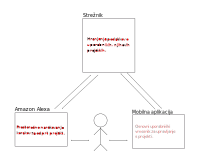
\includegraphics[width=13cm]{plan_simple}
\end{center}
\caption{Preprost načrt sistema}
\label{plan_simple}
\end{figure}


Osnovni uporabniški vmesnik sistema je mobilna aplikacija.
Preko nje se uporabnik v sistem prijavi s svojim uporabniškim računom, ustvarja in odpira svoje delavniške dnevnike.

Delavniški dnevnik oz. projekt sestavljajo naslov, opis dela, opis možnih nevarnosti in seznam korakov postopka.

V odprt projekt lahko uporabnik, enega za drugim, dodaja korake, ki opisujejo potek dela.
Posamezen korak sestavljajo naslov, opis in trajanje.
Uporabnik lahko tudi posname slike in jih doda v odprt projekt kot korak.
% Ker smo želeli ohraniti sistem učinkovit tudi za splošnejše stvari,
Vsi podatki, ki jih uporabnik vnese preko mobilne aplikacije in glasovnega pomočnika, se hranijo na strežniku.

Glasovnega pomočnika smo uporabili kot dodaten uporabniški vmesnik, s katerim lahko uporabnik prostoročno dodaja korake v odprt projekt.

\noindent Z njim smo želeli doseči:
\begin{itemize}
	\item prostoročno narekovnaje besedilnega koraka projekta,
	\item prostoročno odpiranje obrazca za dodajanje koraka v projekt in
	\item prostoročno odpiranje kamere na mobilni napravi.
\end{itemize}


Opredeljeno natančneje, sistem mora uporabniku omogočati ustvarjanje novega opisa tehnološkega postopka in odpiranje ter urejanje obstoječih opisov tehnološkega postopka.

Vsak ustvarjen opis tehnološkega postopka mora imeti naslov, opis dela, opis možnih nevarnosti pri delu in seznam korakov dela, ki ga sestavljajo.

Seznam korakov dela mora podpirati dodajanje novih korakov, spreminjanje vsebine obstoječih korakov, brisanje obstoječih korakov in spreminjanje vrstnega reda korakov.

Posamezen korak mora imeti naslov, opis dela in predvideno trajanje opisanega dela.



\subsection{Smernice razvoja sistema za sestavljanje delavniškega dnevnika}

Pri načrtovanju sistema za sestavljanje opisov tehnoloških postopkov smo se osredotočali predvsem na nasledje točke:
\begin{itemize}
	% \item prekinitve dela, ki jih povzroči uporaba sistema morajo biti čim krajše,
	% \item uporabniški vmesnik odjemalca mora omogočati karseda učinkovito delo,
	\item uporabniški vmesniki sistema (mobilna aplikacija, glasovni pomočnik) morajo biti zamenjljivi,
	\item uporabljene podatke (fotografije, zapiske) se mora hraniti na enem mestu,
	\item sistem mora biti popolnoma funkcionalen brez glasovnega pomočnika.
\end{itemize}

Sistem, ki smo ga implementirali v tej raziskavi, služi kot primer kompleksnejšega sistema, katerega uporabnost bi radi izboljšali z uporabo glasovnega pomočnika.


\subsection{Kaj smo želeli z glasovnim pomočnikom izboljšati?}

Glasovni pomočnik v našem sistemu služi kot uporabniški vmesnik za prostoročno dodajanje korakov v odprt projekt.
Glasovni pomočnik je smiseln način interakcije z računalniškim sistemom v situaciji, kjer uporabnik nima prostih rok ali je fizično oddaljen od naprave.

% Z glasovnim pomočnikom smo poskusili implementirati dodajanje korakov v odprt projekt.

Osnovna funkcionalnost glasovnega pomočnika je prostoročno narekovanje besedila koraka v projektu.
Poleg narekovanja besedila korakov smo implementirali odpiranje obrazcev za dodajanje korakov v projekt in zagon kamere.

\bigbreak 
Glasovni pomočnik v našem sistemu ima naslednje vloge:
\begin{itemize}
	\item za trenutno odprt opis tehnološkega postopka je z njim možno dodajati korake postopka,
	\item z njim je možno odpreti kamero ali obrazec za dodajanje koraka.
\end{itemize}

Raziskava iz leta 2018 \cite{austerjost2018introducing} je pokazala izboljšano učinkovitost pri delu raziskovalcev v kemijskem laboratoriju, v katerega so integrirali glasovne pomočnike.
% Namen raziskave je bil preizkus praktične uporabnosti glasovnih pomočnikov za branje laboratorijskih postopkov po korakih in glasovno upravljanje laboratorijskih instrumentov.
Namen raziskave je bil preizkus praktične uporabnosti glasovnih pomočnikov za branje laboratorijskih postopkov in glasovno upravljanje laboratorijskih instrumentov.
Pozitivni rezultati bi lahko bili ključnega pomena za slabovidne člane laboratorijev.
Kot glasovnega pomočnika so uporabili Amazon Alexo.
Prepoznavanje govora in ukazov je bilo konsistentno in hitro, ne glede na spol uporabnika.
Motnje pri razpoznavanju je povzročal večinoma ozadni hrup.
Povprečna uspešnost prepoznave ukazov je bila 95\%.
Raziskovalci so zabeležili tudi problem moteče kakofonije v laboratoriju, v katerem je več raziskovalcev, ki uporabljajo glasovni nadzor naprav.

\section{Načrt sistema za sestavljanje opisov tehnoloških postopkov}

% Sistem za sestavljanje opisov tehnoloških postopkov smo poimenovali OpenReport. 


Sistem za sestavljanje opisov tehnoloških postopkov smo poimenovali OpenReport. 
Sistem OpenReport (na sliki \ref{plan}) sestavljajo:

\begin{itemize}
	\item strežniški program, 
	\item mobilna aplikacija,
	\item glasovni pomočnik.
\end{itemize}

\begin{figure}[H]
\begin{center}
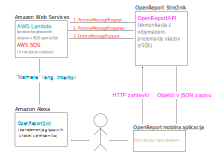
\includegraphics[width=13cm]{plan}
\end{center}
\caption{Visokonivojski načrt sistema}
\label{plan}
\end{figure}

Strežnik v podatkovni bazi hrani uporabnike, opise tehnoloških postopkov in korake.
Uporabnik lahko do podatkov na strežniku dostopa preko odjemalca, ki s strežnikom komunicira preko API.
V našem primeru je to mobilna aplikacija.
Glasovnega pomočnika smo uporabili kot dodatek k mobilni aplikaciji.
Omogoča glasovno upravljanje aplikacije in narekovanje korakov.

\bigbreak
Preko mobilne aplikacije uporabnik lahko:
\begin{itemize}
	\item opravi regsitracijo in prijavo,
	\item ustvari nov delavniški dnevnik,
	\item odpre obstoječe delavniške dnevnike,
	\item ustvarja in ureja korake delavniškega dnevnika,
	\item zajema slike in jih vstavlja v delavniški dnevnik,
	\item briše korake delavniškega dnevnika,
	\item ureja vrstni red korakov delavniškega dnevnika.
\end{itemize}

Za glasovnega pomočnika Amazon Alexa smo razvili \enquote{Skill}, s katerim uporabnik lahko:

\begin{itemize}
	\item v odprto poročilo vstavi dobesedno narekovan korak,
	\item odpre obrazec za dodajanje novega besedilnega koraka,
	\item odpre kamero in obrazec za dodajanje koraka s fotografijo.
\end{itemize}


\subsection{Zasnova aplikacije}

Mobilna aplikacija služi kot osnovni način za interakcijo s strežnikom.

V tej diplomski nalogi preučujemo, ali je možno z vpeljavo glasovnega pomočnika v naš sistem izboljšati učinkovitost tega sistema.
Da bodo rezultati raziskave čim bolj natančni, smo dali učinkovitosti mobilne aplikacije velik poudarek.
Uporabniški vmesnik je bil zasnovan za čim hitrejše delo.
To nam je v zagotovilo, da uporabniški vmesnik aplikacije ni ozko grlo pri pisanju opisov tehnoloških postopkov.

\section{Uporabljene tehnologije}

\subsection{.NET}

.NET \cite{dotnet} je razvojna platforma, razvita s strani Microsofta.
Obsega programske jezike, prevajalnike, orodja in knjižnice, ki omogočajo širok spekter primerov uporabnosti, hkrati pa se ohranja enovitost ozadne kode.

Tehnologije .NET ogrodja, ki smo jih uporabil v tej diplomski nalogi so:
\begin{itemize}
	\item .NET Core - odprtokodna platforma za razvoj spletnih storitev,
	\item Xamarin - ogrodje za razvoj mobilnih aplikacij za najpogostejše mobilne operacijske sisteme (Android, iOS).
\end{itemize}

.NET smo izbrali, ker je zelo dobro integriran z Amazonovim AWS API-jem in je dobro dokumentiran.

\subsection{Xamarin}

Ogrodje Xamarin \cite{xamarin} je odprtokodno orodje za razvoj mobilnih aplikacij, ki ga je razvil Microsoft. 

Z njim je mogoče deliti večino ozadne in ospredne kode med različnimi mobilnimi operacijskimi sistemi. 
Za ozadno kodo se uporablja .NET (C\#), za ospredno kodo pa se uporablja XAML (Extensible Application Markup Language).

Xamarin smo izbrali, da smo lahko strežniški program in mobilno aplikacijo programirali v enakem programskem jeziku (C\#).

\subsection{Amazon Alexa}

% // Besede \enquote{Skill} ne bi prevajal, z enakim razlogom kot ne bi prevajal npr. Python. Gre za ime nekega produkta.

Amazon Alexa je glasovni pomočnik, razvit s strani podjetja Amazon \cite{alexa}.
Za Amazon Alexo smo se odločili, saj ponuja ogrodje za programiranje dodatnih funkcionalnosti, ki se imenuje Alexa Skills Kit.
Poleg tega je Alexo enostavno integrirati z drugimi Amazonovimi spletnimi storitvami, ki smo jih uporabili v tej diplomski nalogi (AWS SQS, AWS Lambda).

% \subsection{Alexa Skill}

Alexine osnovne funkcionalnosti lahko nadgradimo s programi, ki se jim reče \enquote{Skill-i} (na sliki \ref{alexa_architecture}) \cite{alexaskills, alexaarchitecture}.
Da lahko ustvarimo in objavimo \enquote{Skill} rabimo račun Amazon razvijalca (\textit{ang. Amazon Developer Account}).

\begin{figure}[H]
\begin{center}
\includegraphics[width=13cm]{alexa_architecture}
\end{center}
\caption{Arhitektura Alexa \enquote{Skill-a}}
\label{alexa_architecture}
\end{figure}

\noindent \enquote{Skill} sestavljajo:
\begin{itemize}
	\item \textbf{Poziv} - fraza, ki \enquote{Skill} zažene,
	\item \textbf{Namera} - fraze, ki jih \enquote{Skill} razpozna kot funkcije,
	\item \textbf{Krajišče} - omrežni vir, kjer se nahaja ozadna koda \enquote{Skill-a}.
\end{itemize}



Ko Alexa zasliši poziv ali katero od namer, glasovni posnetek pošlje na Amazonov Alexa Voice Service.
Ta s pomočjo glasovnega razpoznavnega modela prepozna uporabnikove ukaze in pošlje poseben zahtevek na krajišče.
To je lahko druga Amazonova storitev (npr. AWS Lambda), storitev na Microsoftovem Azure strežniku ali naš lasten strežnik, dostopen preko javne domene in zaščiten s SSL.

Ko krajišče obdela zahtevo, odgovor pošlje nazaj na Amazon Alexa Server.
Ta odgovor se nato pošlje nazaj na Alexo, ki uporabniku \enquote{izgovori} prejet odgovor.

\subsection{Amazon Web Services}

Amazon Web Services (v nadaljevanju AWS) je skupek oblačnih storitev, ki jih ponuja podjetje Amazon.
Ponuja integracijo s pogostimi programskimi jeziki in ogrodji, kot so Java, .NET, Python in Node.js preko storitve AWS API.
Pri tej diplomski nalogi smo se osredotočili na dva sistema iz skupka AWS.

\subsubsection{Simple Queue Service}

AWS Simple Queue Service (v nadaljevanju SQS) je sistem za pošiljanje tekstovnih sporočil med odjemalci preko Amazonovih strežnikov \cite{sqs}.
Za hranjenje sporočil je potrebno registrirati \enquote{SQS Queue} \textit{(slo. SQS vrsto)}. 
Ta je lahko neurejena vrsta, kjer prejeta sporočila niso nujno urejena po času ustvarjanja, lahko pa je tipa FIFO (first in, first out) \cite{sqsfifo}, pri kateri je zagotovljeno, da dobimo vsa sporočila v vrstnem redu, v katerem so bila poslana.
V sklopu te diplome smo uporabili vrsto tipa FIFO.

To storitev smo uporabili za komunikacijo med Amazon Alexo in OpenReport strežnikom.

\subsubsection{Lambda}

Ozadno kodo za Alexa \enquote{Skill} smo gostili na platformi AWS Lambda, ki je storitev za gostovanje dogodkovno vodene ozadne kode \cite{lambda}.
Za to platformo smo se odločili zaradi dobre integracije z Alexa Skill Kit in razvojnim orodjem Visual Studio.

\section{Strežnik}

Osrednja komponenta sistema OpenReport je strežnik.
Strežnik je zadolžen za delo s podatki uporabnikov in njihovih delavniških dnevnikov.
Odjemalci, ki so nanj povezani, služijo zgolj kot \enquote{uporabniški vmesnik} za prikaz podatkov na strežniku.

Operacije nad podatki, hranjenimi na strežniku, se sprožijo na strani odjemalca in izvedejo na strežniku.

Osnovne naloge strežnika so:
\begin{itemize}
	\item Avtentikacija uporabnikov,
	\item avtorizacija uporabnikovih zahtev,
	\item komunikacija z glasovnim pomočnikom,
	\item hranjenje podatkov o uporabnikih in delavniških dnevnikih in
	\item ponujanje vmesnika, ki ga lahko odjemalci uporabijo za sprožanje operacij nad delavniškimi dnevniki.
\end{itemize}

Za uporabo strežnika za hranjenje podatkov smo se odločili, da lahko do podatkov dostopamo iz različnih naprav preko enotnega vmesnika (API).
To nam omogoča enostavno dodajanje odjemalcev in odpravi podvajanje podatkov.
Če bi podatke hranili na odjemalčevi napravi, bi bil dostop do njih iz druge naprave bistveno otežen.

V našem primeru bosta s strežnikom komunicirala mobilna aplikacija in glasovni pomočnik.
Podatke hranimo v podatkovni bazi, ki jo streže SQL Server.

\subsection{Komunikacija z odjemalci}

Strežnik z odjemalci komunicira preko API.
To metodo smo izbrali zaradi enostavnosti implementacije in možnosti širjenja nabora odjemalcev v prihodnosti.

V našem primeru je bil edini odjemalec mobilna aplikacija.
Odjemalec na definirane funkcijske URL-je (slika \ref{api_routes}) strežnika pošlje HTTP zahtevke.
Če so zahtevki pravilno oblikovani, strežnik izvede predvideno funkcijo in rezultat te funkcije pošlje kot HTTP odgovor nazaj odjemalcu.
Komunikacija med strežnikom in odjemalcem je prikazana z roza barvo na spodnji sliki (slika \ref{plan_server_client}).

\begin{figure}[H]
\begin{center}
\includegraphics[width=8cm]{plan_server_client}
\end{center}
\caption{Komunikacija strežnika z odjemalcem}
\label{plan_server_client}
\end{figure}


\subsection{Podatkovni model}

V sklopu diplomske naloge smo se odločili podatke razdeliti v tri entitete:
\begin{itemize}
	\item uporabnik,
	\item delavniški dnevnik,
	\item korak delavniškega dnevnika.
\end{itemize}

Uporabnik lahko tako sestavlja svoje delavniške dnevnike, vsak delavniški dnevnik pa je sestavljen iz zbirke korakov, ki opisujejo potek dela.

Podatkovna baza hrani tabele \enquote{AspNetUsers}, \enquote{Projects} in \enquote{Notes} (slika \ref{er_diagram}).
Vsak uporabnik lahko ima 0 ali mnogo delavniških dnevnikov (v nadaljevanju tudi projektov).
Vsak projekt ima lahko 0 ali mnogo korakov.

\begin{figure}[H]
\begin{center}
\includegraphics[width=13.5cm]{er_diagram_small}
\end{center}
\caption{ER model podatkovne baze}
\label{er_diagram}
\end{figure}

Uporabnik mora imeti uporabniško ime, katerega uporabi za prijavo in geslo s katerim dokaže, da je to res on.
% Uporabnik mora imeti možnost dodajanja svojih projektov.

Vsak delavniški dnevnik mora imeti naslov, opis in enolični identifikator uporabnika, ki si dnevnik lasti.

Vsak korak delavniškega dnevnika mora imeti naslov, opis, podatke o trajanju in enolični identifikator projekta, ki si korak lasti.


% \noindent Strežnik ima naslednje naloge:
% \begin{enumerate}
% 	\item komunikacija s podatkovno bazo,
% 	\item ponujanje vmesnika, preko katerega lahko odjemalci delajo s podatki v bazi (API),
% 	% \item komunikacija z odjemalcem (mobilno aplikacijo),
% 	\item komunikacija z glasovnim pomočnikom (Amazon Alexa).
% \end{enumerate}


\subsection{Implementacija API}

% Komunikacija med strežnikom in odjemalci poteka preko HTTP po pristopu API (slika \ref{api_routes}).
% Podatki v HTTP sporočilih se zapišejo v format JSON.
API smo uporabili kot vmesnik za komunikacijo med odjemalcem in strežnikom, ki hrani podatke (slika \ref{api_routes}).
Zanj smo se odločili predvsem zaradi enostavnosti implementacije.

Ker lahko sistem uporablja več uporabnikov, smo se odločili implementirati sistema za avtentikacijo uporabnikov in avtorizacijo zahtev.
Avtentikacija z uporabniškim imenom in geslom omogoča preverjanje identitete.
Ko se vzpostavi zaupanje, se prijavljenemu uporabniku dodeli avtorizacijski žeton.
Iz žetona je možno razbrati, za katerega uporabnika gre in katere pravice so mu dodeljene.


\begin{figure}[H]
\begin{center}
\includegraphics[width=13.5cm]{api_routes_small}
\end{center}
\caption{Avtomatsko dokumentiranje funkcijskih URL-jev s Swagger}
\label{api_routes}
\end{figure}

\subsubsection{Registracija in prijava}

Da lahko uporabnik dostopa do svojih delavniških dnevnikov, mora biti avtenticiran.
Vse operacije nad uporabnikovimi delavniškimi dnevniki morajo biti avtorizirane.
Uporabnik sistema mora za uporabo sistema imeti registriran uporabniški račun.
Na ta račun so vezani vsi njegovi delavniški dnevniki.

Preden dobi uporabnik dostop do svojih podatkov, mora vzpostaviti zaupanje s strežnikom.
To doseže s prijavo s pravilnim uporabniškim imenom in geslom.
Če uporabnik še nima računa, se mora registrirati.

Pri registraciji mora odjemalec na strežnik poslati objekt razreda \textit{RegisterUserRequest}.
Odjemalec ga mora poslati na URL \enquote{\texttt{/identity/register}} preko metode POST.
V objektu \texttt{RegisterUserRequest} se nahajata njegov e-mail naslov in geslo v čisti obliki.

\begin{verbatim}
RegisterUserRequest {
    string Email; 
    string Password; 
} 
\end{verbatim}


Ko strežnik prejme ta objekt, ga pošlje v avtentikacijsko storitev.
V tej storitvi preveri, ali uporabnik s tem uporabniškim imenom že obstaja v bazi (je že bil registriran).
Če obstaja, se zabeleži napaka in nadaljnja registracija se prekine.
Če ta uporabnik ne obstaja, se kreira nov objekt razreda \texttt{User}.
Polje \texttt{Password} se šifrira in se skupaj s poljem \texttt{Email} zapiše v ta objekt.
Objekt se nato zapiše v podatkovno bazo v tabelo \texttt{Users}.
Uporabnik pri registraciji dobi tudi svoj enoličen identifikator \texttt{UserID}.

V kolikor se je tekom avtentikacije dogodila kakršna koli napaka, se odjemalcu vrne objekt razreda \texttt{AuthFailedResponse}.
V tem objektu se odjemalcu pošlje seznam vseh napak, ki jih je avtentikacijska storitev zabeležila pri neuspešni registraciji. 

\begin{verbatim}
AuthFailedResponse { 
     IEnumerable<string> Errors; 
}
\end{verbatim}


Če je bila registracija uspešna, se odjemalcu pošlje objekt razreda \texttt{Auth-\\SuccessResponse}.

\begin{verbatim}
AuthSuccessResponse { 
    string UserId; 
    string Token; 
} 
\end{verbatim}


\noindent V polje \texttt{Token} razreda \texttt{AuthSuccessResponse} se zapiše avtorizacijski žeton.
Žeton je tipa JWT ali \textit{JSON Web Token} \cite{jwtinfo}.
Sestavljajo ga e-mail uporabnika, uporabnikov enolični identifikator \texttt{UserID}, čas zapada žetona in tip simetričnega kodiranja, uporabljenega za enkripcijo žetona.

Objekt \texttt{AuthSuccessResponse} se pošlje nazaj odjemalcu.
Odjemalec žeton iz prejetega objekta doda glavi vseh svojih HTTP zahtevkov na OpenReport strežnik.
Strežnik ga uporabi pri poizvedbah po podatkovni bazi.

Prijava poteka podobno.
Uporabnik mora poslati na strežnik objekt \textit{LoginUserRequest}.
Ciljni URL za ta zahtevek je \enquote{\texttt{/identity/login}}.
V objektu \texttt{LoginUserRequest} se nahajata njegov e-mail naslov in geslo.

\begin{verbatim}
LoginUserRequest {
    string Email; 
    string Password; 
} 
\end{verbatim}

Ko strežnik prejme ta objekt, ga pošlje v avtentikacijsko storitev.
V tej storitvi preveri, ali uporabnik s tem e-mail naslovom že obstaja.
Če uporabnik ne obstaja, ali pa je njegovo šifrirano geslo v podatkovni bazi drugačno kot to, kar je v polju \texttt{Password}, se zabeležijo napake in prijava se prekine.
Odjemalec prejme objekt razreda \texttt{AuthFailedResponse}.

Če uporabnik obstaja in se njegovo šifrirano geslo iz polja \texttt{Password} ujema z geslom v podatkovni bazi, je avtentikacija uspešna.
Odjemalec prejme objekt razreda \texttt{AuthFailedResponse}.

V primeru uspešne prijave se avtorizacijski žeton \texttt{Token} generira in pošlje enako kot pri registraciji.

\subsubsection{Operacije z delavniškimi dnevniki}

Strežnik mora podpirati dodajanje, odpiranje in brisanje delavniških dnevnikov za prijavljenega uporabnika.
Pri dodajanju delavniškega dnevnika, se v uporabnikovo zbirko doda nov prazen dnevnik z naslovom in opisom, ki ga vpiše uporabnik.
Pri brisanju se morajo vsi podatki izbrisanega dnevnika odstraniti iz podatkovne baze.
Ko uporabnik odpre katerega od svojih delavniških dnevnikov, mu mora strežnik vrniti ta dnevnik in zbirko korakov, ki mu pripada.

Avtenticiran uporabnik lahko dostopa do svoje zbirke delavniških dnevnikov.
Vsak uporabnik lahko ima nič ali več delavniških dnevnikov.

Vse operacije nad uporabnikovim delavniškim dnevnikom morajo biti avtorizirane.
V kolikor niso, API javi napako \texttt{Bad Request: Not Authorised}.

Ko uporabnik želi ustvariti nov delavniški dnevnik (slika \ref{app_create_new})(v nadaljevanju poglavja \textit{projekt}), mora v mobilni aplikaciji podati naslov, kratek opis projekta in opis možnih nevarnosti.

Te podatke odjemalec zapiše v objekt razreda \texttt{CreateProjectRequest}.

\begin{verbatim}
CreateProjectRequest { 
    string Title;  
    string Description; 
    string Dangers; 
} 
\end{verbatim}

\begin{figure}[H]
\begin{center}
\includegraphics[width=7cm]{app_create_new_small}
\end{center}
	\caption{Ustvarjanje novega projekta v aplikaciji.}
\label{app_create_new}
\end{figure}

\noindent Ta objekt se nato pošlje preko POST metode na strežnik na naslov \texttt{/projects\\/create}.
Storitev za operacije nad projekti nato kreira nov objekt razreda \texttt{Project} s podatki iz prejete zahteve.
V primeru, da je zahteva ustrezno oblikovana in avtorizirana, se projekt zapiše v podatkovno bazo.
Odjemalcu se kot odgovor pošlje ustvarjen objekt tega projekta.

\noindent Razred \texttt{Project} izgleda tako:

\begin{verbatim}
Project { 
    int Id; // unikatni identifikator 
    string Title; 
    string Description; 
    string Dangers; 
    IEnumerable<Note> Notes; // seznam korakov 
    ... 
}
\end{verbatim}

Uporabnik lahko dostopa do katerega koli svojega delavniškega dnevnika.
Do njega dostopa tako, da pošlje avtoriziran GET zahtevek na URL \enquote{\texttt{/projects/\{id\}}}.
Polje \texttt{\{id\}} mora biti unikatni identifikator projekta.

Za izbris projekta mora uporabnik poslati DELETE zahtevo na URL \enquote{\texttt{/projects/\{id\}}}.
Če zahteva ni avtorizirana z ustreznim žetonom, se projekt ne izbriše.

\subsubsection{Operacije nad koraki delavniškega dnevnika}

Korak delavniškega dnevnika opisuje eno od nalog v tehnološkem postopku, ki ga delavniški dnevnik opisuje.
Vsak projekt ima lahko nič ali več korakov.
Vsak korak ima naslov, opis in predvideno trajanje.

Sistem mora podpirati dodajanje korakov v delavniški dnevnik, brisanje spreminjanje vsebine posameznega koraka in spreminjanje vrstnega reda korakov v posameznem delavniškem dnevniku.
Ker lahko delavniški dnevnik vsebuje tudi slikovno gradivo, smo korake ločili na dva tipa: slikovne in besedilne.
Besedilni korak vsebuje naslov, besedilo in trajanje naloge, ki jo opisuje, slikovni pa ima poleg teh lastnosti še fotografijo.

% Korak je lahko izključno tekstovni, lahko pa ima tudi pripadajočo sliko.

Da uporabnik ustvari nov besedilni korak (na sliki \ref{note_image} levo), mora v aplikaciji izpolniti obrazec za dodajanje koraka.
Ta obrazec ima polja za naslov, besedilo in trajanje.
Da uporabnik ta korak vnese, mora poslati objekt razreda \texttt{Note}, preko POST metode, na URL \enquote{\texttt{/projects/\{id\}/addnote}}.
Polje \texttt{\{id\}} mora biti unikatni identifikator projekta, katermu želi dodati korak.

\noindent Razred \texttt{Note} izgleda tako.

\begin{verbatim}
Note { 
    ... 
    string Title; 
    string Text; 
    int Hours; 
    int Minutes;
    int Seconds;
    ...
}
\end{verbatim}

Naslov koraka se zapiše v polje Title, opis v polje Text, trajanje pa se zapiše v polja Hours, Minutes in Seconds.

Ko uporabnik pošlje objekt s podatki nas strežnik, strežnik najprej preveri, če je pošiljatelj poslal avtorizirano zahtevo.
Iz avtorizacijskega žetona strežnik razbere uporabnikov \texttt{UserID}. 
Če je projekt z identifikatorjem \texttt{\{id\}} res v lasti uporabnika z identifikatorjem \texttt{UserID}, se korak doda v zbirko korakov tega projekta.

Slikovni koraki (na sliki \ref{note_image} desno) se v delavniški dnevnik dodajajo na podoben način.
Uporabnik v mobilni aplikaciji odpre kamero in zajame fotografijo, ki se nanaša na korak, ki ga želi ustvariti.
Ko jo zajame, se odpre obrazec za dodajanje naslova, opisa in trajanja koraka s fotografijo.
Ko so podatki vnešeni, se slika zašifrira v znakovni niz po metodi Base64.
Ostali podatki se zapišejo v objekt razreda \texttt{Note}.

Korak, zapisan v objekt razreda \texttt{Note} in v znakovni niz šifrirana slika se zapišeta v objekt razreda \texttt{UploadImageRequest}.
Ta objekt se nato pošlje preko POST metode na URL \enquote{\texttt{/projects/\{id\}/addimage}}.

\begin{verbatim}
UploadImageRequest { 
    Note note; 
    string ImageString; 
}
\end{verbatim}

\begin{figure}[H]
\begin{center}
\includegraphics[width=11cm]{app_note_image}
\end{center}
	\caption{Dodajanje korakov v aplikaciji.}
\label{note_image}
\end{figure}

V tem razredu predstavlja polje \texttt{ImageString} pripadajočo fotografijo, po metodi Base64 šfirirano v znakovni niz.
% Za kodirni algoritem smo uporabili Base64.

Za hranjenje tekstovnih in slikovnih korakov smo zaradi preprostosti implementacije uporabili isti razred (\texttt{Note}).
Tekstovni in slikovni korak se ločita v vrednosti boolean zastavice \texttt{IsImage}.
Tekstovni korak ima to zastavico nastavljeno na vrednost \texttt{false}, slikovni pa \texttt{true}.

\begin{Verbatim}[commandchars=+\[\]]
Note { 
    +underline[bool IsImage;]
    string Title; 
    string Text; 
    int Hours; 
    int Minutes;
    int Seconds; 
    +underline[string Url;] // Lokacija slike na odjemalcu 
    +underline[string ServerUrl;] // Lokacija slike na strežniku
    ... 
}
\end{Verbatim}

Poljema \texttt{Url} in \texttt{ServerUrl} se dodeli vrednost samo pri slikovnih korakih.
Ko se na odjemalcu zajame fotografija, odjemalec nastavi vrednost polja \texttt{Url} na lokacijo ustvarjene fotografije v datotečnem sistemu.

Polje \texttt{ServerUrl} se nastavi šele na strežniku.
Ko strežnik prejme zahtevo za kreiranje slikovnega koraka, se korak \texttt{Note} prebere iz objekta \texttt{UploadImageRequest} in zapiše v podatkovno bazo.
Nato se \texttt{ImageString} dekodira v slikovno datoteko in hrani na strežniku.
Ko se fotografija uspešno zapiše v datotečni sistem, se v polje \texttt{ServerUrl} zapiše lokacija pravkar ustvarjene datoteke.
Spremembe se hranijo v podatkovni bazi.

\subsubsection{Urejanje in brisanje in korakov v projektu}

Uporabnik lahko korake, ki pripadajo njegovim delavniškim dnevnikom spreminja.
Spreminja lahko njihovo vsebino, naslov in trajanje.

Po končanem urejanju besedilnih korakov, mora odjemalec poslati avtorizirano PUT zahtevo na URL \enquote{\texttt{/projects/\{pid\}/update/\{nid\}}}.
Telo zahteve mora vsebovati objekt razreda \texttt{Note}, ki ga je uporabnik spremenil.

Pri spreminjanju vsebine slikovnih korakov mora odjemalec poslati avtorizirano PUT zahtevo na naslov \enquote{\texttt{/projects/\{pid\}/update/\{nid\}/image}}.
Telo te zahteve mora vsebovati objekt razreda \texttt{UploadImageRequest}.
V objektu \texttt{UploadImageRequest} mora biti polje \texttt{Note} objekt, ki ga želimo posodobiti.
Polje \texttt{ImageString} mora biti šifrirana slika, ki bo zamenjala prejšnjo sliko.
Slika mora biti šifrirana po metodi Base64.

Pri izbrisu koraka iz projekta, mora uporabnik poslati avtorizirano zahtevo na URL \enquote{\texttt{/projects/\{pid\}/delete/\{nid\}}}.
V tem primeru je polje \texttt{\{pid\}} unikatni identifikator projekta, v katerem se nahaja korak, \texttt{\{nid\}} pa unikatni identifikator objekta \texttt{Note}, ki ga želimo izbrisati.
V kolikor ima ta objekt \texttt{Note} postavljeno zastavico \texttt{IsImage} na \texttt{true}, se poleg zapisa v bazi izbriše tudi pripadajoča slikovna datoteka.


\subsubsection{Spreminjanje vrstnega reda korakov v projektu}

% Sistem mora podpirati tudi 
Uporabnik lahko korakom v svojih delavniških spreminja vrstni red prikaza.
Izbran korak lahko zamakne za poljubno število mest proti začetku ali koncu seznama.
Položaj koraka \texttt{Note} v seznamu lahko razberemo iz atributa \texttt{Position}.
Prvi korak ima \texttt{Position} 0, drugi 1, itd.

\begin{Verbatim}[commandchars=+\[\]]
Note { 
    int Id; 
    +underline[int Position;]
    bool IsImage;  
    string Title; 
    string Text;
    int Hours; 
    int Minutes;
    int Seconds;
    string Url;
    string ServerUrl;
}
\end{Verbatim}

Pri dodajanju korakov v projekt se obstoječe korake projekta razvrsti po vrednosti polja \texttt{Position}.
Najdemo največjo vrednost tega polja, ki se v seznamu pojavi in ji prištejemo 1.
Nato to vrednost priredimo polju \texttt{Position} novo kreiranega koraka.

Ko uporabnik želi spremeniti pozicijo koraka v projektu, moramo poslati zahtevo PUT na URL \enquote{\texttt{/projects/\{pid\}/\{nid\}/\{positions\}}}.

Polje \texttt{\{pid\}} predstavlja unikatni identifikator projekta, v katerem se nahaja korak.
Polje \texttt{\{nid\}} predstavlja unikatni identifikator koraka \texttt{Note}.
Polje \texttt{\{positions\}} pa prestavlja število mest za kolikor ga želimo prestaviti.
To število je lahko pozitivno ali negativno celo število.
Negativna vrednost \texttt{\{positions\}} prestavi korak proti začetku seznama, pozitivna pa proti koncu.

\subsubsection{Izvoz projektov}

Sistem omogoča izvoz projektov v druge računalniške formate.
Izvožene datoteke lahko služijo kot sredstvo za pomoč pri prenosu zapisanih podatkov v druge računalniške sisteme ali kot varnostna kopija.
Projekt lahko uporabnik izvozi v dva formata, v besedilno datoteko in HTML dokument.

V besedilno datoteko ga uporabnik izvozi, tako, da pošlje avtorizirano GET zahtevo na URL \enquote{\texttt{/projects/\{id\}/export/text}}.
V HTML dokument ga uporabnik izvozi, tako, da pošlje avtorizirano GET zahtevo na URL \enquote{\texttt{/projects/\{id\}/export/html}}.

Pri izvozu v besedilno datoteko, storitev za upravljanje projektov na strežniku ustvari novo besedilno datoteko.
Najprej vanjo vpiše naslov in opis projekta ter možne nevarnosti pri delu.
Nato uredi korake po vrednosti stolpca \texttt{Position} in besedila korakov eno za drugim zapiše v datoteko.
Pri slikovnih korakih se, poleg besedila, zapiše tudi lokacija pripadajoče fotografije.

Pri izvozu v HTML dokument (slika \ref{export_html}) se naslov projekta zapiše kot HTML naslov H1, opis projekta kot naslov H2, koraki pa kot HTML odstavki.
V HTML dokumentu lahko prikažemo poleg besedila slikovnih korakov tudi slike.

\begin{figure}[H]
\begin{center}
\includegraphics[width=13cm]{export_html}
\end{center}
\caption{Projekt, izvožen v HTML dokument}
\label{export_html}
\end{figure}

Lokacija izvožene datoteke se nahaja v polju \texttt{FolderLocation} v razredu \texttt{Project}.
Privzeta lokacija, ki se nastavi ob kreiranju projekta je 
\\\enquote{\texttt{C:/users/\$USER/Public Documents/OpenReport}}.

\begin{Verbatim}[commandchars=+\[\]]
Project {
    int Id; 
    string Title; 
    string Description; 
    string Dangers; 
    +underline[string FolderLocation;] // lokacija pripadajočih datotek 
    IEnumerable<Note> Notes; 
    ... 
}
\end{Verbatim}

\subsection{Komunikacija strežnika z glasovnim pomočnikom}

Da lahko strežnik obdela ukaze, ki jih je uporabnik izgovoril Amazon Alexi, jih mora odgovore glasovnega pomočnika najprej prejeti.

\begin{figure}[H]
\begin{center}
\includegraphics[width=13cm]{plan_sqs_server_alexa}
\end{center}
\caption{Komunikacija med strežnikom in glasovnim pomočnikom preko SQS}
\label{plan_sqs_server_alexa}
\end{figure}


Strežnik z glasovnim pomočnikom Amazon Alexa komunicira (slika \ref{plan_sqs_server_alexa}) preko storitve Simple Queue Service (SQS) iz sklopa storitev Amazon Web Services.
To komunikacijo smo implementirali tako, da Amazon Alexa rezultate obdelanih glasovnih ukazov odloži v SQS vrsto, strežnik pa jih iz te vrste prebere.

SQS vrsta, tipa first-in-first-out \cite{sqsfifo}, ki smo jo uporabili, je sklad tekstovnih sporočil.
Nanjo lahko odlagamo nova sporočila ter beremo in brišemo obstoječa sporočila .


Glasovni pomočnik od uporabnika prejme izgovorjen glasovni ukaz.
Na podlagi tega ukaza, glasovni pomočnik na SQS vrsto odloži tri različna besedilna sporočila:
\begin{itemize}
	\item \textbf{\enquote{addnote}},
	\item \textbf{\enquote{addimage}},
	\item \textbf{\enquote{\{narekovano besedilo\}}},
\end{itemize}

% \bigbreak
Strežnik periodično prejema sporočila iz SQS vrste.
Ko sporočilo prejme, na podlgi njegove vsebine izvede eno od treh možnih funkcij.

\begin{itemize}
	\item Sporočilo \enquote{addnote} sporoči strežniku, naj na odjemalcu odpre obrazec za dodajanje besedilnega koraka.
	\item Sporočilo \enquote{addimage} sporoči strežniku, naj na odjemalcu odpre kamero in obrazec za dodajanje slikovnega koraka.
	\item Sporočilo \enquote{\{narekovano besedilo\}} sporoči strežniku, naj vsebino tega sporočila doda odprtemu projektu kot tekstovni korak.
\end{itemize}

V sporočilu \enquote{\{narekovano besedilo\}} se nahaja besedilo, ki ga je glasovni pomočnik razpoznal kot dobesedni narek koraka.
Primer takšnega sporočila je \enquote{this is a literal dictation} ali \enquote{prepare the table}.

\subsubsection{Utemeljitev uporabe SQS}

Prenos sporočil med Amazon Alexo in strežnikom smo realizirali z uporabo storitve AWS SQS.
Pri uporabi SQS je prenos podatkov resda manj učinkovit kot pri direktni povezavi preko spletne vtičnice (\textit{ang. Web Socket}).

Glavni faktor, zaradi katerega smo se odločili za uporabo AWS SQS, je, da z dodatno plastjo za hranjenje sporočil, dosežemo enostavno zamenjljivost glasovnega pomočnika.

Pri morebitni menjavi glasovnega pomočnika, strežniškega programa ne bi spreminjali.
Potrebno bi bilo le implementirati program za novega glasovnega pomočnika, da na AWS SQS odlaga sporočila v strežniku razumljivem formatu (\enquote{addnote}, \enquote{addimage},...).

\subsubsection{Zahtevanje in izpust glasovnega pomočnika}

En OpenReport strežnik podpira delo z enim samim glasovnim pomočnikom.
Tega pomočnika lahko uporabnik \enquote{zahteva} za lastno uporabo in ga po uporabi \enquote{izpusti}.
Ko se uporabnikova zahteva potrdi, lahko glasovnega pomočnika uporablja pri sestavljanju delavniškega dnevnika.
Po končani uporabi lahko uporabnik glasovnega pomočnika izpusti, kar omogoči drugim uporabnikom, da ga lahko zahtevajo za svoje delo.

Če ima določen uporabnik nase vezanega pomočnika, vidimo po vrednosti zastavice \texttt{UsesVoiceAssistant}.
Ta se nahaja v uporabnikovem objektu razreda \texttt{User}.
Uporabnik pomočnika uporablja, če je zastavica nastavljena na \texttt{True}.

Ko uporabnik odpre katerega od svojih projektov, se identifikator tega projekta nastavi v polje \texttt{LastOpenedProjectId} v njegovem objektu razreda \texttt{User}.

Zahtevki, ki jih strežniku pošlje Alexa preko SQS vrste, se navezujejo na projekt s tem identifikatorjem.

\begin{Verbatim}[commandchars=+\[\]]
User : IdentityUser {
    string Id; 
    string Email;
    string Password; 
    IEnumerable<Project> Projects;
    ... 
    +underline[int LastUsedProjectId;]
    +underline[bool UsesVoiceAssistant;]
}
\end{Verbatim}

\subsubsection{Delovanje}

Komunikacija med strežnikom in glasovnim pomočnikom je prikazana z rdečo barvo na spodnji sliki (slika \ref{plan_sqs_server}).

\begin{figure}[H]
\begin{center}
\includegraphics[width=13cm]{plan_sqs_server}
\end{center}
\caption{Komunikacija med strežnikom in SQS}
\label{plan_sqs_server}
\end{figure}

Na strežniku OpenReport teče storitev za komunikacijo z glasovnim pomočnikom.
Ta storitev vsakih pet sekund na SQS pošlje zahtevek \texttt{RecieveMessageRequest}.

\begin{Verbatim}[commandchars=+\[\]]
RecieveMessageRequest {
    AttributeName 
    MaxNumberOfMessages 
    QueueUrl 
    WaitTimeSeconds
    ... 
} 
\end{Verbatim}

AWS SQS kot odgovor vrne objekt tipa \texttt{RecieveMessageResponse}.

\begin{Verbatim}[commandchars=+\[\]]
RecieveMessageResponse {
    IEnumerable<Message> Messages;
    ...
}
\end{Verbatim}

V tem odgovoru se nahaja seznam sporočil, ki čakajo na sprejem iz SQS vrste.
V kolikor je v odgovoru vsaj eno sporočilo, pregledamo telo vseh sporočil. 

Ko strežnik sporočila sprejme, jih mora izbrisati iz SQS vrste.
Če jih sproti ne izbriše, iz FIFO vrste ne more brati najnovejših sporočil, ampak le 5 najstarejših.

Sporočila izbriše iz SQS vrste z zahtevkom \texttt{DeleteMessageRequest}.
Ta zahtevek hrani referenco na sporočilo, ki ga želimo izbrisati iz SQS vrste.
AWS SQS storitev v odgovor vrne \texttt{DeleteMessageResponse}, a v tej diplomski nalogi tega odgovora ne uporabimo več.

Zahtevki, ki jih strežnik prejme od glasovnega pomočnika se odražajo na zadnjem projektu, ki ga uporabnik z glasovnim pomočnikom odpre.
\begin{itemize}
	\item Zahtevek \enquote{\texttt{addnote}} nastavi zastavico \enquote{\texttt{NoteRequest}} na \texttt{true},
	\item zahtevek \enquote{\texttt{addimage}} nastavi zastavico \enquote{\texttt{ImageRequest}} na \texttt{true},
	\item zahtevek \enquote{\texttt{\{narekovano besedilo\}}} nastavi zastavico \enquote{\texttt{AlexaNoteRequest}} na \texttt{true} in prejeto besedilo doda projektu kot korak.
\end{itemize}

\begin{Verbatim}[commandchars=+\[\]]
Project { 
    int Id; 
    string Title; 
    string Description; 
    string Dangers; 
    string FolderLocation; 
    IEnumerable<Note> Notes; 
    +underline[bool NoteRequest;] 
    +underline[bool ImageRequest;] 
    +underline[bool AlexaNoteRequest;] 
}
\end{Verbatim}


Če je vsebina prejetega sporočila enaka \texttt{addnote}, storitev preveri, kateri uporabnik ima trenutno nase vezanega glasovnega pomočnika.
Nato v projektu, ki ga je nazadnje odprl, nastavi vrednost zastavice \texttt{NoteRequest} na \texttt{true}.


Če je vsebina enaka \enquote{\texttt{addimage}}, storitev preveri, kateri uporabnik ima trenutno nase vezanega glasovnega pomočnika.
Nato v projektu, ki ga je nazadnje odprl, nastavi vrednost zastavice \texttt{ImageRequest} na \texttt{true}.

Če vsebina prejetega sporočila ni enaka \enquote{\texttt{addimage}} ali \enquote{\texttt{addnote}}, pomeni, da je prejeto sporočilo dobesedno narekovan korak.
Kot prej, storitev preveri, kateri uporabnik ima nase vezanega glasovnega pomočnika.
Nato v projektu, ki je nazadnje odprl, nastavi vrednost zastavice \texttt{AlexaNoteRequest} na \texttt{true}.
Poleg tega ustvari nov objekt razreda \texttt{Note}, ki ima naslov \enquote{Voice note}, vsebina pa je telo prejetega sporočila.
Nov objekt se nato vstavi v zadnji odprt projekt.



\section{Implementacija Alexa \enquote{Skill-a}}

Alexa \enquote{Skill} je program, ki glasovnemu pomočniku Amazon Alexa doda funkcionalnosti.
Alexo in zasnovan \enquote{Skill} smo uporabili kot dodaten uporabniški vmesnik za upravljanje z mobilno aplikacijo.

\noindent Z njim smo želeli doseči:
\begin{itemize}
	\item prostoročno narekovnaje besedilnega koraka,
	\item prostoročno odpiranje obrazca za dodajanje korakov v odprt projekt in
	\item prostoročno odpiranje kamere in dodajanje slikovnega koraka v projekt.
\end{itemize}



Ko Alexa zasliši poziv \enquote{\textit{make a report note}}, se naš \enquote{Skill} začne izvajati.

Vsak nadaljnji ukaz, ki ga uporabnik izreče, preden se \enquote{Skill} preneha izvajati, se primerja s frazami namer.
Namere se uporabljajo za zagon funkcij, ki smo jih implementirali v ozadni kodi \enquote{Skill-a} (slika \ref{plan_alexa_sqs}).
V našem \enquote{Skill-u} smo definirali tri glavne namere:

\begin{itemize}
	\item \texttt{TakeNoteIntent},
	\item \texttt{OpenTextNoteFormIntent},
	\item \texttt{OpenImageNoteFormIntent}.
\end{itemize}

\begin{figure}[H]
\begin{center}
\includegraphics[width=6cm]{plan_alexa_sqs}
\end{center}
\caption{Načrt komunikacije Alexe, AWS Lambda in AWS SQS}
\label{plan_alexa_sqs}
\end{figure}

\texttt{TakeNoteIntent} (slika \ref{TakeNoteIntent}) se zažene, ko po pozivu uporabnik izreče \enquote{\texttt{take note \{besedilo\}}} ali \enquote{\texttt{note \{besedilo\}}}.
Polje \texttt{\{besedilo\}} je besedilna spremenljivka, v katero \enquote{Skill} hrani razpoznano besedilno vsebino koraka.
V primeru, da uporabnik izreče \enquote{\textit{note unscrew the backplate}}, je vrednost spremenljivke \texttt{\{besedilo\}} \enquote{unscrew the backplate}.

\begin{figure}[H]
\begin{center}
\includegraphics[width=13cm]{intent_literal}
\end{center}
\caption{TakeNoteIntent v Alexa Developer nadzorni plošči}
\label{TakeNoteIntent}
\end{figure}

\texttt{TakeNoteIntent} v ozadni kodi \enquote{Skill-a} zažene funkcijo, ki ustvari novo SQS sporočilo.
V telo tega sporočila funkcija vstavi vrednost spremenljivke \texttt{\{besedilo\}} in ga pošlje v SQS vrsto.
To SQS sporočilo prebere strežnik in ga kot korak vstavi v odprt projekt.
\enquote{Skill} zatem vrne uporabniku odgovor \enquote{Noted!} in se preneha izvajati.

\texttt{OpenTextNoteFormIntent} se zažene, ko po pozivu uporabnik izreče \enquote{\texttt{create a text note}}.

\texttt{OpenTextNoteFormIntent} v ozadni kodi \enquote{Skill-a} zažene funkcijo, ki ustvari novo SQS sporočilo.
V telo tega sporočila funkcija vstavi besedilo \enquote{\texttt{addnote}} in ga pošlje v SQS vrsto.
To SQS sporočilo prebere strežnik in mobilni aplikaciji sporoči, naj odpre obrazec za dodajanje novega besedilnega koraka.
\enquote{Skill} zatem vrne uporabniku odgovor \enquote{Opening the form!} in se preneha izvajati.


\begin{figure}[H]
\begin{center}
\includegraphics[width=8cm]{intent_text}
\end{center}
\caption{OpenTextNoteFormIntent}
\label{OpenTextNoteFormIntent}
\end{figure}

\texttt{OpenImageNoteFormIntent} se zažene, ko po pozivu uporabnik izreče \enquote{\texttt{take a picture}}.

Ta namera v krajišču \enquote{Skill-a} zažene funkcijo, ki ustvari novo SQS sporočilo.
V telo tega sporočila funkcija vstavi besedilo \enquote{\texttt{addimage}} in ga pošlje v SQS vrsto.
To SQS sporočilo prebere strežnik in mobilni aplikaciji sporoči, naj odpre kamero.
\enquote{Skill} zatem vrne uporabniku odgovor \enquote{Launching camera!} in se preneha izvajati.

\begin{figure}[H]
\begin{center}
\includegraphics[width=8cm]{intent_image}
\end{center}
\caption{OpenImageNoteFormIntent}
\label{OpenImageNoteFormIntent}
\end{figure}

\subsection{Izvajanje \enquote{Skill-a} po korakih}

Alexa \enquote{Skill} se začne izvajati, ko uporabnik izreče poziv \enquote{\textit{make a report note}}.
Alexa posnet govorni ukaz pošlje na Amazon Alexa Service \cite{skillexecution}.
Tam se s pomočjo NLU razpoznavnega modela poskusi pretvoriti v znakovni niz.
Ta znakovni niz se primerja z vsemi definiranimi pozivnimi frazami za \enquote{Skill-e}, ki so vezani na naš Amazon račun.

Če Amazon Alexa Service uporabnikov glasovni ukaz razpozna kot \enquote{make a report note}, se začne izvajati OpenReportAlexaSkill.
V krajišče \enquote{Skill-a} se pošlje zahteva tipa \texttt{LaunchRequest}.

Krajišče nastavimo v Alexa Developer nadzorni plošči (slika \ref{skill_endpoint}).
Krajišče je lahko AWS Lambda funkcija, lahko pa je naš lasten strežnik, dostopen preko javne domene in zaščiten z SSL.
Krajišče je v našem primeru gostovan na storitvi AWS Lambda.
Ob prejetju \texttt{LaunchRequest} krajišče našega \enquote{Skill-a} vrne vprašanje What now?.

\begin{figure}[H]
\begin{center}
\includegraphics[width=13cm]{skill_endpoint}
\end{center}
\caption{Krajišče OpenReportAlexaSkill-a v Alexa Developer nadzorni plošči}
\label{skill_endpoint}
\end{figure}

Naslednji glasovni ukaz, po zagonu \enquote{Skill-a}, se primerja s frazami za namere.
Če se ukaz ujema z frazami, ki zaženejo katero od namer TakeNoteIntent, OpenTextNoteFormIntent ali OpenImageNoteFormIntent, se na krajišče pošlje zahteva tipa \texttt{IntentRequest}.

Iz prejetega \texttt{IntentRequest}-a nato dobimo ime namere.
Na podlagi imena prejete namere ločimo, ali gre za TakeNoteIntent, OpenTextNoteFormIntent ali OpenImageNoteFormIntent in zaženemo funkcije, opisane v prejšnjem poglavju.

% Oris obdelave poziva \enquote{Skill-a} in namere \texttt{TakeNoteIntent} je prikazan s spodnjo sliko (slika \ref{skill}).
% 
% \begin{figure}[H]
% \begin{center}
% 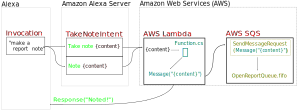
\includegraphics[width=13.5cm]{skill_2}
% \end{center}
% \caption{Načrt Alexa Skilla}
% \label{skill}
% \end{figure}

\subsection{Ovire pri izdelavi Alexa \enquote{Skill-a}}

Pri implementaciji Alexa \enquote{Skill-a} smo naleteli na največ težav v sklopu te raziskave.

Prva je bila jezikovne narave, saj Alexa ne podpira prepoznavanja slovenskega jezika.
Zato smo se odločili za uporabo angleškega jezika.

Naslednja težava je bila definicija pozivne fraze.
Fraze, kot so \enquote{take a note} ali \enquote{take a picture} so že rezervirane v sklopu Alexinih privzetih funkcionalnosti.
To pomeni, da jih za naš \enquote{Skill} ne moremo uporabiti.

Izogibati smo se morali tudi frazam, ki so bile rezerviranim frazam podobne (npr. \enquote{open report note} itd.).
Tudi take fraze so se velikokrat razpoznale kot rezervirane fraze.

Težavo je predstavljala izbira poziva, ki je bil hkrati kratek, intuitiven in se ni napačno interpretiral v poziv privzetih funkcionalnosti.
Poziv \enquote{make a report note} je bila najboljši kompromis, ki smo ga našli.

Težavo je predstavljalo tudi razpoznavanje dolgih stavkov, še posebej, če se ti niso ujemali z definiranimi frazami namer.
To je zelo omejilo možnost narekovanja besedila korakov s pomočjo Amazon Alexe.

Naslednjo težavo je predstavljal čas, ki ga je Alexa porabila za interpretacijo definiranih glasovnih ukazov.
Za procesiranje glasovnih ukazov je porabila v povprečju od 3 do 6 sekund.

\section{Implementacija mobilne aplikacije}


Za osnovni uporabniški vmesnik našega sistema smo uporabili mobilno aplikacijo.
Preko aplikacije se uporabnik lahko registrira in prijavi v sistem, dodaja, briše, odpira in izvaža svoje delavniške dnevnike.
V delavniške dnevnike lahko dodaja korake, ki opisujejo delo, jih briše, spreminja vsebino ter ureja vrstni red.

Preko mobilne aplikacije lahko tudi zahteva in izpusti glasovnega asistenta.
Z mobilno napravo lahko zajema fotografije in jih v delavniške dnevnike dodal kot slikovno gradivo.

Mobilno aplikacijo smo uporabili kot primer odjemalca za naš strežnik (slika \ref{plan_server_client}).

Do strežnika dostopa preko API vmesnika.
Zahtevki se prenašajo preko HTTP protokola.

Mobilno aplikacijo smo se odločili razviti s tehnologijo Xamarin.
Razlogi za to so predvsem naše dobro poznavanje tehnologije in enostavna integracija z ostalimi tehnologijami iz .NET sklopa.


\subsection{Pristop}
Pristop razvoja aplikacije, ki smo ga uporabili za programiranje aplikacije, se imenuje \enquote{Model View View-Model} (v nadaljevanju MVVM).
Pri tem pristopu aplikacijo razdelimo na tri dele (slika \ref{mvvm}).

\textbf{Model} je del, kjer definiramo elemente naše podatkovne logike (opis tehnološkega postopka, korak, uporabnik,...).

\textbf{View} je uporabniški vmesnik, ki ga vidi uporabnik.

\textbf{ViewModel} pa se uporablja, da se poveže funkcije uporabniškega vmesnika in modela (podatkovne logike) ter po potrebi preoblikuje podatke.

Rezultat upoštevanja tega pristopa je čista koda, ki nima prepletenih elementov med ozadno kodo in uporabniškim vmesnikom.
\enquote{Model} vsebuje le abstrakcijo naših podatkov in podatkovno logiko.
Ti podatki se v \enquote{ViewModel-u} pretvorijo v obliko, ki bo prikazana uporabniku.
\enquote{View} pa nato servira pripravljene podatke uporabniku v obliki grafičnih elementov.

Na spodnji sliki lahko vidimo oris pristopa MVVM (slika \ref{mvvm}) \cite{mvvmimage}.

\begin{figure}[H]
\begin{center}
\includegraphics[width=11cm]{mvvm}
\end{center}
	\caption{Shema pristopa MVVM}
\label{mvvm}
\end{figure}

\subsection{Povezava na strežnik, prijava in registracija uporabnika}

Uporabnik se mora za uporabo sistema OpenReport najprej povezati na OpenReport strežnik.
Ob zagonu mobilne aplikacije, uporabnika pričaka stran za povezavo na strežnik.
V besedilno polje mora vpisati IP naslov strežnika.
Ta naslov bomo v nadaljevanju podpoglavja označevali z \texttt{naslovstrežnika}.

% // slika povezavne strani

\begin{figure}[H]
\begin{center}
\includegraphics[width=4cm]{app_connect}
\end{center}
\caption{Povezavna stran}
\label{app_connect}
\end{figure}


Za kreiranje in avtorizacijo HTTP zahtevkov v okviru aplikacije skrbi storitev za komunikacijo s strežnikom (razred \texttt{OpenReportServerCommunicati-\\onService.cs}).
Storitev se registrira ob zagonu aplikacije po metodi Dependency Injection.
Za to metodo registracije storitev smo se odločili, saj omogoča enostavno uporabo instanc registriranih storitev kjerkoli v aplikaciji.

Ko uporabnik pritisne na gumb \enquote{Connect}, se preveri, ali je naslov pravilno vnešen.
Če je, storitev za komunikacijo s strežnikom pošlje neavtorizirano GET zahtevo na \enquote{\texttt{naslovstrežnika}/connect}. 
Če je na tem naslovu res OpenReport strežnik, se kot odgovor odjemalcu pošlje boolean vrednost \texttt{true}.

Storitev za komunikacijo s strežnikom si nato hrani vrednost \texttt{naslovstre-\\žnika} kot predpono vseh nadaljnjih zahtevkov.

Ob neuspešnem poskusu povezave, se uporabniku na strani prikaže opis napake.
Če je poskus uspešen, se stran za povezavo na strežnik zapre.

Prikaže se stran za prijavo.
Na tej strani uporabnik vpiše svoje uporabniško ime ali geslo, lahko pa odpre stran za registracijo računa.

\begin{figure}[H]
\begin{center}
\includegraphics[width=8cm]{app_login}
\end{center}
	\caption{Prijavna stran pred poskusom prijave (levo), in po uspešnem poskusu prijave (desno)}
\label{app_login}
\end{figure}

Ko je uporabnik uspešno povezan na strežnik, se mora za dostop do svojih delavniških dnevnikov prijaviti ali registrirati.
Za prijavo in registracijo skrbi avtentikacijska storitev (razred \texttt{IdentityService.cs}).
Ta storitev je, enako kot storitev za komunikacijo s strežnikom, registrirana po metodi Dependency Injection.
Uporabljamo jo lahko, ko je storitev za komunikacijo uspešno vzpostavila komunikacijo s strežnikom.

Poskus prijave poteka tako, avtentikacijska storitev uporabniško ime in geslo zapiše v objekt razreda \texttt{LoginUserRequest}.
Uporabniško ime in geslo se vneseta na prijavni strani.

\begin{Verbatim}[commandchars=+\[\]]
LoginUserRequest {
    string Email; 
    string Password;
}
\end{Verbatim}

Nato se objekt \texttt{LoginUserRequest} pošlje na strežnik.
Odjemalec ga pošlje na URL \enquote{\texttt{/identity/login}} preko POST metode.
Strežnik ob uspešni avtentikaciji vrne objekt razreda \texttt{AuthSuccessResponse}.
Iz tega objekta uporabnik prebere svoj avtorizacijski žeton.
Ta žeton hrani avtentikacijska storitev.
Komunikacijska storitev ta žeton doda v glavo nadaljnjih HTTP zahtevkov.

Če je avtentikacija neuspešna, strežnik vrne objekt razreda \texttt{AuthFailed-\\Response}, v katerem je podan opis napake.
Ta opis napake se nato uporabniku izpiše na prijavni strani.

Stran za registracijo (slika \ref{app_register}) je podobna strani za prijavo, le, da ima dve vnosni polji za vpis gesla.
Vrednost v obeh poljih za geslo mora biti enaka, da se lahko uporabnik registrira.

Registracijski zahtevek se pošlje na strežnik na URL \enquote{\texttt{/identity/regis-\\ter}}.
Zahtevek je objekt razreda \texttt{RegisterUserRequest}.

\begin{Verbatim}[commandchars=+\[\]]
RegisterUserRequest {
    string Email; 
    string Password;
}
\end{Verbatim}

\begin{figure}[H]
\begin{center}
\includegraphics[width=4cm]{app_register}
\end{center}
	\caption{Registracijska stran}
\label{app_register}
\end{figure}

\subsection{Ustvarjanje, brisanje in odpiranje projektov}

Po prijavi lahko uporabnik odpre stran s seznamom njegovih delavniških dnevnikov, imenovano Dashboard.
Na tej strani se prikažejo:
\begin{itemize}
	\item seznam vseh njegovih projektov, 
	\item gumbi za izbris posameznega projekta,
	\item gumb za dodajanje novega projekta in
	\item gumb za zahtevanje in izpust glasovnega pomočnika.
\end{itemize}

\subsubsection{Ustvarjanje novega projekta}

Za ustvarjanje novega delavniškega dnevnika (slika \ref{app_newproject}), mora uporabnik odpreti stran za dodajanje projektov.
Na tej strani mora vpisati naslov projekta (\texttt{Title}), kratek opis (\texttt{Description} in našteti možne nevarnosti pri delu \texttt{Dangers}.

Te tri vrednosti se zapišejo v objekt razreda \texttt{CreateProjectRequest}.
\begin{Verbatim}[commandchars=+\[\]]
CreateProjectRequest {
    string Title;
    string Description;
    string Dangers;
}
\end{Verbatim}

Ta objekt nato storitev za komunikacijo s strežnikom pošlje preko metode POST na URL \enquote{\texttt{/projects/create}}.
Strežnik v odgovor vrne objekt razreda \texttt{Project}, ki ga je zahtevek ustvaril.

Nov projekt se nato prikaže v seznamu vseh uporabnikovih projektov na strani \enquote{My Projects}, kjer ga lahko uporabnik odpre ali izbriše.

\begin{figure}[H]
\begin{center}
\includegraphics[width=13cm]{app_newproject}
\end{center}
	\caption{Postopek ustvarjanja novega projekta po korakih.}
\label{app_newproject}
\end{figure}

\subsubsection{Izbris projekta}

Da uporabnik izbriše delavniški dnevnik, mora na strani \enquote{My projects} ob željenem projektu pritisniti gumb z ikono smetnjaka.
Pritisk na ta gumb sporoči storitvi za komunikacijo s strežnikom, naj pošlje avtoriziran DELETE zahtevek na URL \enquote{\texttt{/projects/\{id\}/delete}}.
Strežnik ob uspešnem izbrisu projekta odjemalcu vrne kopijo izbrisanega projekta.

\subsection{Zahtevanje in izpust glasovnega pomočnika}
Storitev za upravljanje z glasovnim pomočnikom (\texttt{VoiceAssistantService.cs}) skrbi za zahtevanje in izpust glasovnega pomočnika.
% Za zahtevanje in izpust glasovnega pomočnika v mobilni aplikaciji skrbi storitev za upravljanje z glasovnim pomočnikom (razred \texttt{VoiceAssistantService.cs}).
Ta storitev se registrira ob začetku izvajanja aplikacije, nato pa počaka, da avtentikacijska storitev uspešno opravi prijavo uporabnika.
Ob prijavi uporabnika preveri, ali ta uporablja glasovnega pomočnika.
To doseže tako, da pošlje GET zahtevek na URL \enquote{\texttt{/users/current}}.
Strežnik vrne objekt \texttt{User}, ki pripada prijavaljenemu uporabniku.
Storitev preveri vrednost boolean atributa \texttt{UsesVoiceAssistant}.

Če ima uporabnik vrednost polja \texttt{UsesVoiceAssistant} nastavljeno na \texttt{true}, lahko ima glasovnega pomočnika vezanega nase.

Če ima uporabnik vrednost polja \texttt{UsesVoiceAssistant} nastavljeno na \texttt{false}, mora uporabo glasovnega pomočnika zahtevati.
To naredi tako, da pošlje avtoriziran PUT zahtevek na URL \enquote{\texttt{/users/requestva}}.

Če noben drug prijavljen uporabnik nima polja \texttt{UsesVoiceAssistant} nastavljenega na \texttt{true}, se njegova zahteva odobri.
V njegovem objektu \texttt{User} se nastavi vrednost \texttt{UsesVoiceAssistant} na \texttt{true}.

Če ima kateri od uporabnikov to polje nastavljeno na \texttt{true}, zahteva ne bo odobrena.
V tem primeru mora uporabnik, ki zahteva pomočnika počakati, da uporabnik, ki pomočnika uporablja, pomočnika izpusti.
Ko si pomočnika ne lasti nobeden drug uporabnik, ga lahko veže nase.

Izpust pomočnika dosežemo, da uporabnik, ki pomočnika trentuno uporablja, pošlje avtoriziran PUT zahtevek na URL \enquote{\texttt{/users/releaseva}}.

V mobilni aplikaciji zahtevanje in izpust pomočnika nadziramo na \enquote{Dashboard} strani, s pritiskom na ikono mikrofona (slika \ref{app_alexa_yesno}).

\begin{figure}[H]
\begin{center}
\includegraphics[width=7cm]{app_alexa_yesno}
\end{center}
	\caption{Gumb v obeh stanjih}
\label{app_alexa_yesno}
\end{figure}

\subsection{Odpiranje in sinhronizacija projekta}

Ko uporabnik iz seznama delavniških dnevnikov izbere projekt, ki ga želi odpreti, storitev za komunikacijo s strežnikom pošlje na URL \enquote{\texttt{/projects/\{id\}/notes}} zahtevek GET.
Polje \texttt{\{id\}} je unikatni identifikator željenega projekta.

Storitev za projekte (razred \texttt{ProjectService.cs}) nato prejet odgovor, razreda \texttt{Project}, hrani.
Vse korake, ki pripadajo temu projektu, se hrani v seznam tipa ObservableCollection.
Ta tip seznama smo izbrali, saj je v ogrodju Xamarin nad njim najlažje opravljati zamenjevalne operacije.
Seznam se nato prikažem na strani za upravljanje s projektom.

Storitev nato začne s periodično sinhronizacijo projekta.
Storitev za projekte na URL \enquote{\texttt{/projects/\{id\}/nonotes}} pošlje avtoriziran GET zahtevek.
Strežnik vrne objekt razreda \texttt{Project} s praznim seznamom korakov.
Vse, kar storitev za projekte pri sinhronizaciji gleda, je vrednost zastavic \texttt{NoteRequest}, \texttt{ImageRequest} in \texttt{AlexaNoteRequest}.

Na \texttt{true} nastavljena zastavica \texttt{NoteRequest} odpre obrazec za dodajanje novega besedilnega koraka v projekt.

Na \texttt{true} nastavljena zastavica \texttt{ImageRequest} odpre obrazec za dodajanje nove fotografije v projekt.

Na \texttt{true} nastavljena zastavica \texttt{AlexaNoteRequest} storitvi za projekte sporoči, naj pošlje GET zahtevek na URL \enquote{\texttt{/projects/\{id\}/notes}}.
Polje \{id\} mora biti unikatni identifikator odprtega projekta.
V odgovor prejme objekt razreda \texttt{Project}, vključno s seznamom vseh korakov, ki mu pripadajo.
V prejetem seznamu je namreč tudi narekovan korak.
Storitev za projekte primerja, katerega od korakov še nima v svoji zbirki.
Ko ta korak najde, ga doda v svoj ObservableCollection.

Ko se projekt sinhronizira, storitev za projekte pošlje na strežnik PUT zahtevo na URL \enquote{\texttt{/project/last/closerequests}}.
Ta zahteva nastavi vrednost zastavic \texttt{NoteRequest}, \texttt{ImageRequest} in \texttt{AlexaNoteRequest} na \texttt{false}.


\subsection{Dodajanje in brisanje zapiskov}

Ko ima uporabnik projekt odprt, lahko vanj dodaja korake, jih briše, ureja in jim spreminja vrstni red.
Doda lahko tekstovni korak ali korak s fotografijo.

\begin{figure}[H]
\begin{center}
	\includegraphics[width=9cm]{app_note_image}
\end{center}
	\caption{Stran za dodajanje in urejanje korakov}
\label{app_note}
\end{figure}

Pri dodajanju besedilnega koraka mora uporabnik v vnosnem obrazcu (slika \ref{app_note}) podati naslov koraka (\texttt{Title}), opis koraka (\texttt{Text}) ter trajanje v urah, minutah in sekundah.
Ti podatki se nato hranijo v objektu razreda \texttt{Note}.
Ta objekt storitev za projekte vključi v objekt razreda \texttt{AddNoteRequest} in ga pošlje storitvi za komunikacijo s strežnikom.

\begin{Verbatim}[commandchars=+\[\]]
AddNoteRequest { 
    Note note; 
}
\end{Verbatim}

Storitev za komunikacijo s strežnikom pošlje ta objekt na strežnik.
Pošlje ga na URL \enquote{\texttt{/projects/\{id\}/addnote}} preko metode POST.
Polje \texttt{\{id\}} mora biti unikatni identifikator projekta, v katerega želimo korak vstaviti.
Če je vstavljanje v projekt uspešno, strežnik odjemalcu pošlje v odgovor kopijo dodanega objekta \texttt{Note}.

Storitev za projekte nato ta korak doda svoji zbirki korakov.

Pri vstavljanju slikovnih korakov je postopek vstavljanja podoben.
Ko uporabnik odpre stran za dodajanje slikovnega koraka, se zažene privzeta aplikacija za kamero.
Ko uporabnik fotografijo posname, se ta prikaže na strani z vnosnim obrazcem (slika \ref{app_note}).
Slika se na mobilni napravi hrani v mapi \enquote{\texttt{Pictures/\{naslov projekta\}}}, v uporabnikovem domačem direktoriju.
Uporabnik ima na vnosnem obrazcu možnost sliko ponovno posneti ali jo odstraniti.

Uporabnik mora v vnosnem obrazcu podati naslov koraka (\texttt{Title}), opis koraka (\texttt{Text}) ter trajanje v urah, minutah in sekundah.

Uporabnik mora nato pritisniti gumb za vstavljanje slikovnega koraka v projekt.
Storitev za upravljanje s projektom fotografijo zakodira v znakovni niz po metodi Base64.
Storitev za komunikacijo s strežnikom zakodirano fotografijo in novo ustvarjen objekt razreda \texttt{Note} vključi v objekt tipa \texttt{UploadImageRequest}.

\begin{Verbatim}[commandchars=+\[\]]
UploadImageRequest {
    Note note;
    string ImageString; 
}
\end{Verbatim}

Novo nastali zahtevek \texttt{UploadImageRequest} se nato avtorizira z JWT avtorizacijskim žetonom in pošlje na URL \enquote{\texttt{/projects/\{id\}/addimage}}.
Polje \texttt{\{id\}} mora biti unikatni identifikator projekta, v katerega želimo korak vstaviti.
Če je vstavljanje v projekt uspešno, strežnik odjemalcu pošlje v odgovor kopijo pravkar vstavljenega objekta \texttt{Note}.


\subsubsection{Uporaba kamere v Xamarin}

% https://github.com/jamesmontemagno/MediaPlugin

Za uporabo kamere v ogrodju Xamarin smo uporabili vtičnik Xam.Plugin.Media \cite{xampluginmedia}.
Vtičnik je licensiran pod MIT licenco.

Zanj smo se odločili, saj podpira zajem fotografij s privzeto aplikacijo za zajemanje fotografij.
Izbiramo lahko tudi kvaliteto zajete fotografije.

Pri zajemu slike najprej preverimo, ali imamo zadostne pravice.
Imeti moramo pravice za dostop do shrambe, dostop do fotografij in dostop do kamere.

Fotografijo nato zajamememo z metodo \texttt{TakePictureAsync}.
Kreirano fotografijo nato preberemo in znotraj aplikacije hranimo v objektu razreda ImageSource.
Fotografijo v tej obliki lako prikažemo v XAML z grafičnim elementom Image.
Lahko jo tudi zakodiramo v znakovni niz in pošljemo na strežnik.


\subsection{Izvoz projekta}

Uporabnik lahko projekt izvozi v človeško berljivo obliko na strežnik v dva različna formata: besedilno datoteko (.txt) in HTML dokument.

\begin{figure}[H]
\begin{center}
	\includegraphics[width=4cm]{app_project_export}
\end{center}
	\caption{Stran za izvoz projektov}
\label{app_project_export}
\end{figure}

Če želi uporabnik izvoziti projekt kot besedilno datoteko, storitev za komunikacijo s strežnikom pošlje POST zahtevek na URL \enquote{\texttt{/project/\{id\}/export/text}}.
Če želi uporabnik izvoziti projekt kot HTML dokument, storitev za komunikacijo s strežnikom pošlje POST zahtevek na URL \enquote{\texttt{/project/\{id\}/export/html}}.

% \section{Testiranje sistema OpenReport}

% Sistem OpenReport smo po končani implementaciji testirali.
% Testiranje je bilo izvedeno tako, da smo s sistemom OpenReport sestavili delavniški dnevnik za čiščenje mehanske tipkovnice.
% 
% Najprej smo zagnali aplikacijo in se povezali na strežnik.
% Povezava na strežnik je bila uspešna.
% Če strežnik ni bil dosegljiv, se aplikacija ni ustavila.
% 
% Nato smo se prijavili z uporabniškim imenom \enquote{user@example.com} in geslom \enquote{string}.
% Ob napačno vpisanih podatkih je strežnik javil napako, ki se je izpisala pod prijavnim obrazcem.
% // TODO slika
% 
% Po uspešni prijavi smo na strani Dashboard zahtevali uporabo glasovnega asistenta.
% Nato smo odprli stran za dodajanje novega projekta (na sliki \ref{testproject} levo).
% Tam smo vpisali ime projekta, opis in možne nevarnosti (na sliki \ref{testproject} v sredini).
% 
% \begin{figure}[H]
% \begin{center}
% 	\includegraphics[width=13.5cm]{app_newproject}
% \end{center}
% 	\caption{Sestavljanje testnega delavniškega dnevnika za čiščenje tipkovnice.}
% \label{testproject}
% \end{figure}
% 
% Ko smo delavniški dnevnik ustvarili, smo začeli z dodajanjem korakov, ki so opisovali posamezne faze dela.
% 
% Testirali smo dodajanje korakov preko uporabniškega vmesnika aplikacije.
% Odprianje obrazca za dodajanje besedilnega koraka s pritiskom na gumb v aplikaciji ni povzročalo težav.
% Odprianje obrazca za dodajanje slikovnega koraka s pritiskom na gumb v aplikaciji ni povzročalo težav.
% 
% // TODO nadaljuj




% \subsection{Testne situacije}
% 
% Pripravili smo štiri testne situacije.
% 
% \begin{enumerate}
% 	\item Izdelava testnega opisa tehnološkega postopka \textbf{brez uporabe glasovnega pomočnika}
% 		\begin{enumerate}
% 			\item brez premora med koraki in
% 			\item z 90 sekundnim premorom med koraki.
% 		\end{enumerate}
% 	\item Izdelava testnega opisa tehnološkega postopka \textbf{z uporabo glasovnega pomočnika}
% 		\begin{enumerate}
% 			\item brez premora med koraki in
% 			\item z 90 sekundnim premorom med koraki.
% 		\end{enumerate}
% \end{enumerate}
% 
% Z 90 sekundnim premorom smo simulirali delo na izdelku.
% Med premorom vpišemo testne podatke v obrazec za dodajanje koraka.
% Po 90 sekundnem premoru korak vstavimo v poročilo.
% 
% \subsubsection{Testno poročilo}
% Testno poročilo mora vsebovati 4 tekstovne korake in enega slikovnega.
% Pri situacijah z uporabo Alexe, mora uporabnik obrazce za korake odpreti z glasovnim ukazom.
% 
% \subsection{Metoda testiranja in vpliv na hipotezo}
% 
% Testne situacije brez premorov so služile za preverjanje hitrosti dela.
% Hipotezo bomo potrdili, če bomo pisanje testnega poročila končali prej \emph{z uporabo Alexe} kot brez nje.
% 
% Če bo uporaba Alexe podaljšala čas pisanja, bomo hipotezo deloma ovrgli in prešli na drugo stopnjo testiranja.
% V drugi stopnji dodamo prejšnjemu postopku 90 sekundni premor med koraki.
% Ta premor simulira delo na izdelku.
% 
% Če bomo v tej situaciji poročilo z Alexo pisali enako hitro kot brez Alexe, hipoteza ostane delno ovržena.
% Če bo pisanje z Alexo počasnejše, kljub premorom, pa se bo hipotezo v celoti ovrglo.
% 
% \subsubsection{Testni koraki}
% 
% Testni koraki simulirajo delo na delovnem mestu, kjer se moramo za uporabo mobilnega telefona oddaljiti od delovnega mesta.
% 
% Testni korak za dodajanje besedilnega koraka je potekal tako:
% \begin{enumerate}
% 	\item premik do mobilnega telefona (3 metre),
% 	\item odpiranje obrazca za dodajanje besedilnega koraka,
% 	\item vpis besedila \enquote{Test step text},
% 	\item nastavitev trajanja na 10 minut,
% 	\item vstavljanje koraka,
% 	\item odmik od mobilnega telefona (3 metre).
% \end{enumerate}
% 
% \noindent Testni korak za dodajanje slikovnega koraka je potekal tako:
% \begin{enumerate}
% 	\item premik do mobilnega telefona (3 metre),
% 	\item odpiranje obrazca za dodajanje slikovnega koraka,
% 	\item zajem slike,
% 	\item vpis besedila \enquote{Test step text},
% 	\item nastavitev trajanja na 10 minut,
% 	\item vstavljanje koraka,
% 	\item odmik od mobilnega telefona (3 metre).
% \end{enumerate}
% 
% Pri situacijah z uporabo Amazon Alexe smo glasovne ukaze začeli izgovarjati, ko smo se začeli premikati proti mobilni napravi.
% 
% \subsection{Rezultati testiranja in ugotovitve}
% 
% \noindent\begin{tabular}{p{0.2\textwidth}|p{.3\textwidth}|p{.4\textwidth}}    
%   {\bf } & {\bf brez premorov}                             & {\bf z 90 sekundnimi premori} \\ \hline
%   {\bf brez Alexe} & 1 minuta 51 sekund & 7 minut 30 sekund \\
%   {\bf z Alexo} & 2 minuti 31 sekund & 7 minut 30 sekund \\
% \end{tabular}
% 
% \bigbreak
% \bigbreak
% % \noindent Iz tega sklepamo, da je hipoteza
% 
% Meritve časa pisanja poročil so pokazale, da je uporaba sistema OpenReport brez Amazon Alexe hitrejša v situacijah brez 90 sekundnih premorov.
% To našo hipotezo delno ovrže.
% V situacijah z 90 sekundnimi premori, je zapis korakov s pomočjo Amazon Alexe trajal enako dolgo kot brez nje.
% To našo hipotezo pusti delno ovrženo.
% 
% Testiranje zaključujemo z ugotovitvijo, da v situacijah brez premorov, Amazon Alexa dela ni pospešila.
% Hkrati pa smo ugotovili, da ga v testni situaciji s premori ni občutno ovirala.
% 
% Iz uporabniškega stališča prinese uporaba glasovnega pomočnika v proces interakcije z računalniškim sistemom novo dimenzijo.
% V našem primeru smo lahko zahtevo za odpiranje vnosnega obrazca v mobilni aplikaciji izvedli že na poti do naprave.

% Ta način bi pohitril delo, če bi lahko glasovni ukaz izgovorili in obdelali na poti do mobilne naprave.

% V naprednejših izvedbah računalniških sistemov z upravljanjem preko glasovnega pomočnika, bi na tak način lahko olajšali delo slabovidnim in gibalno omejenim posameznikom.


\section{Ovrednotenje funkcionalnosti}


% Primerjali smo pisanje opisa tehnološkega postopka na list papirja, s pisarniškim programom in s sistemom OpenReport.
% Sistem OpenReport smo testirali z uporabo Amazon Alexe in brez uporabe Amazon Alexe.
Sistem OpenReport smo po končani implementaciji testirali. 
Mobila aplikacija in strežnik sta izpolnila pričakovanja.

Z mobilno aplikacijo se je bilo možno povezati na strežnik.
Registracija in prijava v sistem preko mobilne aplikacije nista povzročala težav.
Brez težav je delovalo tudi zahtevanje in izpust glasovnega pomočnika Amazon Alexe na strani Dashboard.

Delavniške dnevnike je bilo brez težav možno dodajati, odpirati in brisati.

Možnost dodajanja besedilnih korakov v delavniški dnevnik se je izkazala za smiselno za manjše opombe.
Možnost dodajanja slikovnih korakov v delavniški dnevnik pa se je izkazala za smiselno pri pomembnejših opornih točkah.

Naslove, trajanje in besedilo korakov delavniških dnevnikov smo naknadno spreminjali brez težav.
Urejanje vrstnega reda korakov je delovalo brez težav.
Tudi brisanje korakov delavniškega dnevnika ni povzročalo težav.

Možnost izvoza delavniškega dnevnika v druge formate lahko olajša tudi prenos podatkov v druge računalniške programe.

% Hitrost uporabe sistema se z uporabo glasovnega pomočnika ni izboljšala.
% Kljub temu se je uporaba Alexe kot alternativnega uporabniškega vmesnika izkazala za smiselno 

\bigbreak

Alexa \enquote{Skill} smo testirali tako, da smo vsako frazo namere izgovorili 20-krat in beležili, kolikokrat se je razpoznala pravilno.
Pri dobesednem narekovanju koraka smo testiranje opravili dvakrat.
Prvič smo testirali s stavkom \enquote{\textit{this is a voice note}}, drugič pa s stavkom \enquote{\textit{backplate removal takes about three minutes}}.
\begin{itemize}
	\item Alexa je ukaz \enquote{\textit{take a picture}} pravilno razpoznala v 18 od 20 testnih izgovorjav.
	\item Ukaz \enquote{\textit{create a text note}} je pravilno razpoznala v 17 od 20 testnih izgovorjav.
	\item Ukaz \enquote{\textit{note this is a voice note}} je pravilno razpoznala v 3 od 20 testnih izgovorjav.
	\item Ukaza \enquote{\textit{note backplate removal takes about three minutes}} ni pravilno razpoznala v nobeni od 20 testnih izgovorjav.
\end{itemize}
Pod pričakovnanji se je izkazalo dobesedno narekovanje besedila glasovnemu pomočniku.
Rezultati testiranja razpoznavanja glasovnih ukazov so nam pokazali, da v našem primeru, Alexa veliko bolje razpoznava fraze, ki se z definirano frazo namere v celoti ujemajo, kot tiste, ki nimajo velike stopnje ujemanja.

% Hitrost uporabe sistema se z uporabo glasovnega pomočnika ni izboljšala.
Dodajanje slikovnih in besedilnih korakov, s pomočjo glasovnega ukaza, se je izkazalo za delno uspešno.
% Uporaba Amazon Alexe dela ni pospešila, je pa 
Za uporabno se je izkazalo predvsem, ko mobilnega telefona med delom nismo imeli na dosegu roke.
Kljub temu je problem prikazovalo dejstvo, da je izgovorjava poziva, fraz namer in čakanje na obdelavo zahtev, trajalo v povprečju 18 sekund.


Odklepanje mobilnega telefona, ki ga imamo v dosegu rok in ga lahko dosežemo brez presedanja ter odpiranje forme za dodajanje korakov je trajalo v povprečju 4 sekunde.
Odklepanje mobilnega telefona, ki je oddaljen tri metre ter odpiranje forme za dodajanje korakov je trajalo povprečju 8 sekund.

% \chapter{Možnosti nadaljnega razvoja}

% Glavna šibka točka sistema OpenReport je bil glasovni pomočnik Amazon Alexa.


% Boljšo uporabniško izkušnjo bi dosegli tudi s krajšimi prekinitvami za procesiranje ukaza.
% Ker Amazon Alexa procesira ukaz na oddaljenem strežniku, so večsekundne prekinitve prikazovale precejšnjo oviro.


%  Veliko bolje bi bilo tudi uporabiti algoritme za razpoznavanje govora brez opore definiranih fraz.

\chapter{Zaključek}

Sistem, razvit v sklopu diplomske naloge zajema funkcionalosti, ki uporabniku omogočajo sestavljanje delavniških dnevnikov.
Sestavljajo ga strežnik, mobilna aplikacija in glasovni pomočnik Amazon Alexa.
Uporabnik lahko v delavniške dnevnike dodaja preproste tekstovne korake.
Z uporabo mobilne aplikacije lahko zajame fotografije in jih v delavniški dnevnik vstavi kot slikovno gradivo.

Ta sistem je služil kot primer sistema, ki ga želimo izboljšati z uporabo glasovnega pomočnika.
Naš namen je bil poenostaviti delo s sistemom, z uvedbo glasovnega pomočnika Amazon Alexe.
Implementirali smo odpiranje kamere in obrazca za dodajanje korakov z glasovnim pomočnikom.
Kljub uspešni implementaciji, je bil čas, potreben za izgovorjavo in obdelavo glasovnih ukazov, predolg, da bi poskus izboljšave bil popolnoma uspešen.
Za neuspešno se je izkazalo glasovno narekovanje vsebine koraka delavniškega dnevnika.
Z Amazon Alexo ni bilo mogoče razpoznati daljših, variirajočih glasovnih ukazov.

V možne izboljšave sistema smo na prvo mesto uvrstili preizkus drugih glasovnih pomočnikov, npr. Google Assistant \cite{googleass}.
% Smiselno bi bilo tudi primerjati Amazon Alexo z lastnim glasovnim pomočnikom.
%Hitrejše upravljanje z aplikacijo bi lahko dosegli z pomočnikom, ki bi lahko razpoznal ukaze z eno samo frazo in ne kombinacijo dveh, kot Amazon Alexa.
Druga smiselna izboljšava je izvoz delavniških dnevnikov v več različnih standardnih formatov, kot so npr. XSL.

Mobilna aplikacija in strežniški program sta zadovoljila pričakovanja in lahko že v trenutnem stanju služita kot referenca za primerjavo učinkovitosti Amazon Alexe in drugih glasovnih pomočnikov.

Kljub nekaterim težavam z uporabo glasovnega pomočnika, je očitno, da je tehnologija glasovnih pomočnikov zelo primeren način za nadzor računalniških sistemov na daljavo.
Poleg tega ponuja veliko možnosti za slepe, slabovidne in gibalno omejene posameznike, ki imajo težave z interakcijo z računalnikom.




\newpage %dodaj po potrebi, da bo številka strani za Literaturo v Kazalu pravilna!
\ \\
\clearpage
\addcontentsline{toc}{chapter}{Literatura}

\printbibliography

\end{document}
